%=========================================================================
\makeatletter
\renewcommand*\env@matrix[1][*\c@MaxMatrixCols c]{%
  \hskip -\arraycolsep
  \let\@ifnextchar\new@ifnextchar
  \array{#1}}
\makeatother

\newcommand{\footlabel}[2]{%
    \addtocounter{footnote}{1}%
    \footnotetext[\thefootnote]{%
        \addtocounter{footnote}{-1}%
       ~\refstepcounter{footnote}\label{#1}%
        #2%
    }%
    $^{\ref{#1}}$%
}

\newcommand{\footref}[1]{%
    $^{\ref{#1}}$%
}

\chapter{Introduction}
\label{chapter:introduction}
\textit{This chapter describes the motivation leading to the presentation of this thesis and how is it related to the SLAM\textunderscore frontend\footnote{SLAM\textunderscore frontend, a collection of applications processing sensor outputs and generating inputs for the SLAM++ graph optimizer \url{http://sourceforge.net/projects/slamfrontend/}} and SLAM++\footnote{SLAM++, high -performance nonlinear least squares solver for graph problems \url{http://sourceforge.net/projects/slam-plus-plus/}} libraries developed at Faculty of Information Technology, Brno University of Technology. The objectives of the thesis and the subjects included in this document are briefly explained. The chapter ends describing the overall structure and contents of the remaining of the thesis.}

\vspace{.5cm}
Nowadays we have means to record our surroundings as we perceive it using cameras. However, it has been proven difficult to process such information digitally. Even automated analysis of the 2D information like typeset books is not a trivial problem and far from being mastered. When it comes to 3D, the problem gets much more difficult. Scanning 3D objects reliably is nowadays possible in laboratory conditions, but there are hard limits like the size of the object, its structure or surface and material properties. Also the laboratory equipment used is much more expensive and physically larger compared to its 2D counterpart. This thesis tries to address these problems by allowing user to create 3D model from multiple pictures of an object of interest from various sources. Such 3D model, even though it may be inaccurate, has number of applications. It can be used by archaeologists to preserve cultural heritage, by architects for spatial planning, by entertainers to create 3D models and virtual reality, by engineers to replicate existing 3D objects or in robotics to navigate and interact with the 3D world. One important point, especially for professional use, is that many of the tools presented in chapter~\ref{chapter:the-state-of-the-art} are using cloud based processing. This clashes with licensing and security, because copyrighted images could be uploaded to another country, misused, etc. This concern applies for both medical uses and creative industries.

The process of creating 3D models usually consists of two parts: scanning the object and reconstruction of the model. There are three main approaches how to scan physical object: contact, active non-contact  and passive non-contact scanners. The contact 3D scanners probe the subject through physical touch. The active non-contact scanners use a light in forms of laser or X-ray to scan the object while the passive non-contact scanners are using either multiple images from different angles, images with varying lighting conditions or silhouettes extruded from image with contrasted background. In this thesis we will be particularly interested in scanning objects using multiple images from various cameras. The pipeline of the transformation from 2D images to the 3D models consists of 6 steps: 1) keypoints detection 2) feature extraction  3) feature matching 4) feature and camera tracks building 5) camera initialization and pose estimation 6) structure computation and finally 7) structure refinement. In principle, the algorithm firstly finds points of interests in every image and tries to match them. Once matched the camera positions can be estimated and the structure implemented as a series of 3D points called point cloud. Up till this point we use the SLAM\textunderscore frontend framework which implements some of the pose estimation algorithms. The SLAM++ will then be used for bundle adjustment (BA) as it offers a Nonlinear Least Square solver. Because the process is quite difficult, the resulting 3D structure contains a lot of noise and has to be filtered and segmented before a polygonal model can be created. There is number of tools available for either manual processing of point cloud data, like MeshLab\cite{meshlab}, or the whole process can be automatized using framework like the Point Cloud Library (PCL)~\cite{PCL}.

This thesis aims to identify challenges and propose solutions of three-dimensional reconstruction from a set of two-dimensional images leading to creation of a software, that can do so automatically. The objective is to reduce the correspondence problem between each two images and study the camera modelling and calibration. An accurate estimation of the camera model and correspondence allows us to compute three-dimensional information from a two-dimensional image sequence. In order to eliminate artefacts the input set of images, especially the ones obtained from internet, will have to be filtered to contain only daytime images, without any repetitive watermarks, the image set should be consistent season-wise and contain as little reflective surfaces as possible. Also we are trying to avoid images that are too generic and contain little to none features. Another key goal of this thesis is providing the reader with a complex insight on existing software, how does it work and what are the reconstruction approaches. Lastly formulating and explaining the problem, and the background, using suitable mathematical apparatus.

The study of the geometry involved in multiple camera vision systems should allow us to present an application that can from a set of two-dimensional images reconstruct 3D scene depicted by the images.

The thesis consists of 6 chapters. The chapter~\ref{chapter:the-state-of-the-art} introduces the reader to the current state of the art libraries and programs used in the process of the estimation of the three-dimensional structure from two-dimensional image sequences. Firstly, it discusses existing bundle adjustment (BA) and structure from motion (SfM) solutions, like VisualSFM, Photosynth, OpenMVG and Bundler, and elaborates on the output of these programs and libraries. Later some of them will be used as a benchmark for the implemented application. Some of the mentioned programs, will be used for the final application performance and effectiveness evaluation. Lastly the chapter focuses on the state-of-the-art feature detectors, extractors and matchers, built in the SLAM\textunderscore frontend (and OpenCV) and aims to compare theirs efficiency and performance.

In the chapter~\ref{chapter:methodology} the whole 3D reconstruction process is thoroughly discussed and step by step explained. First the general pipeline is outlined and each step briefly explained.  Second, the camera model is presented and how the distinct camera parameters affect the reconstruction. The chapter also focuses on algorithms for structure evaluation and pose estimation as well as the 3D reconstruction approaches.

The chapter~\ref{chapter:implementation} introduces the design of our application. It covers the whole pipeline starting with the datasets acquisition and camera calibration scripts and programs which outputs are the inputs for our software. However, the main focus of this chapter is on the key data structures and algorithms we have designed and implemented as well as the one provided by the SLAM\textunderscore frontend and SLAM++ frameworks.

The chapter~\ref{chapter:experiments} evaluates the implemented solution on an artificial and real scenes by means of the algorithms described in chapter~\ref{chapter:implementation}. In the beginning of the chapter the datasets used for the evaluation are introduced and their distinct characteristics described. Next, the chapter evaluates different feature detectors, extractors and matchers and elaborates which are suitable for our task and why. Lastly, the chapter presents qualitative results obtained from our program as well as other existing solutions, their evaluation and comparison to reference values where available as well as some complexity and resources consumption evaluation.

Finally, chapter~\ref{chapter:conclusion} summarizes this document by discussing achieved goals and outlining the further work.

\chapter{The State of the Art}
\label{chapter:the-state-of-the-art}
\textit{The following chapter presents to the reader existing implementation of the bundle adjustment and structure from motion techniques. Some of the applications and libraries described will be used as a benchmark for the final solution. The rest of the chapter focuses on the state of the art detectors, extractors and matchers which will be further surveyed in the chapter~\ref{chapter:experiments} in order to choose the best suited combinations for our problem, reconstruction of historic landmarks.}

\section{Existing 3D Reconstruction Applications}
\label{sec:existing_3D_reconstruction_solutions}
There are two image-based 3D reconstruction techniques based on estimating the position of the 3D points in the environment; structure from motion (SfM) and bundle adjustment (BA). The structure from motion tracks the image features from the image sequences obtained by a moving camera. The problem requires camera calibration or an automatic camera parameters re-estimation. If the input image sequence consists of images from multiple cameras with unknown, and often different camera with different intrinsic parameters (like images from Flickr), the 3D reconstruction technique is called bundle adjustment. Both of these techniques are similar, but generally SfM assumes small displacements, images taken from one camera and sequential image datasets, while bundle adjustment works with an unstructured heap of images from multiple cameras.

Bundle adjustment and structure from motion are very similar with simultaneous localization and mapping in robotics (SLAM). In order to deal with the inherent uncertainty, they are formulated as estimation problems and can be elegantly solved using nonlinear least squares (NLS). This is in general not an easy task, and remains a bottleneck in many large-scale computer vision applications.
% Citation of the Ila's work

The problem of creating 3D reconstruction from a set of images has been addressed by many research groups. In this section we will talk about few of the widely known solutions. All of the programs discussed implement a subset of the bundle adjustment pipeline briefly introduced in previous chapter~\ref{chapter:introduction}.

\subsection*{Photosynth}
Photosynth\footnote{Photosynth - Capture your world in 3D, \url{https://photosynth.net}} is a software application developed by Microsoft. It is based on Photo Tourism, a research project by University of Washington graduate student Noah Snavely. Formerly the Photosynth was a 3D reconstruction software, however, in the current version the output of the web application is not a point cloud nor 3D model but an animation of morphing images or panorama. While it still works with images from various sources, the best result is achieved by importing photos from a single camera. Once imported, user has to choose the camera trajectory from four predefined options: spin, panorama, wall or walk. 

The Photosynth technology is using an interest point detection and matching algorithm developed by Microsoft Research which is similar in function to SIFT detector. Detected features are then matched between images and by analysing subtle differences in the relationships between the features (angle, distance, etc.), the program identifies the 3D position of each feature, as well as the position and angle at which each photograph was taken. Everything is processed by Microsoft's servers and, once finished, pushed to the website or desktop/mobile application. There are little to none information about the whole process as this is a commercialized technology.

\begin{figure}[ht]
	\begin{center}
		\includegraphics[keepaspectratio,width=\textwidth]{fig/Photosynth.png}
	\end{center}
	\caption{The Photosynth output for the Červená Lhota Castle (will be introduced in section~\ref{sec:experiments-datasets}) in transition between several morphed images.}
	\label{fig:photosynth}
\end{figure}

\subsection*{VisualSFM}
The Chungchang Wu's Visual Structure from Motion System\footnote{VisualSFM : A Visual Structure from Motion System, \url{http://ccwu.me/vsfm/index.html}} is a GUI application for 3D reconstruction using structure from motion. The reconstruction system is modular and integrates several of other projects: SIFT on GPU (SiftGPU), Multicore Bundle Adjustment, and Towards Linear-time Incremental Structure from Motion. VisualSFM eploits multicore parallelism (both CPU and GPU) for feature detection\footnote{Changchang Wu, SiftGPU: A GPU Implementation of Scale Invariant Feature Transform (SIFT), \url{http://cs.unc.edu/~ccwu/siftgpu}, 2007}, feature matching, and bundle adjustment~\cite{www:multicore-ba}. For dense reconstruction, the program supports Dr. Yasutaka Furukawa's Patch-based Multi-view Stereo Software (PMVS)~\cite{pmvs} and Clustering Views for Multi-view Stereo (CMVS)~\cite{cmvs} tool chain. It can also prepare data for Michal Jancosek's CMPVS~\cite{book:cmpmvs} - Multi-View Reconstruction Software which can create textured polygonal model given camera parameters and set of perspective images. In addition, the output of VisualSFM is natively supported by Mathias Rothermel and Konrad Wenzel's Photogrammetric Surface Reconstruction from Imagery - SURE~\cite{www:sure}.

The software follows the overall 3D reconstruction pipeline; It detects features using SIFT detector and SIFT extractor, matches feature pairs, creates camera tracks, estimates the camera model for each image, removes images' distortion and then runs the dense reconstruction. Most of these parts are done using other libraries mentioned before. The output files of feature extraction and matching are stored as a binary files and are loaded if provided to save processing time. This enables use of other than built-in extractors and matcher, but the format is not widely supported. The whole model is then stored in the N-View Match file format (NVM\footnote{VisualSFM : A Visual Structure from Motion System - Documentation, \url{http://ccwu.me/vsfm/doc.html\#nvm}}) which can contain number of models with cameras, 3D points and associated PLY models (polygon file format, also known as Stanford Triangle Format\footnote{PLY - Polygon File Format, \url{http://paulbourke.net/dataformats/ply/}}). Tutorial on a 3D reconstruction using VisualSFM can be found in appendix~\ref{visualsfm:reconstruction}.

\begin{figure}[ht]
	\begin{center}
		\includegraphics[keepaspectratio,width=\textwidth]{fig/VisualSFM.png}
	\end{center}
	\caption{The VisualSFM application GUI with sparse reconstruction of the Červená Lhota Castle (will be introduced in section~\ref{sec:experiments-datasets}).}
	\label{fig:visualsfm}
\end{figure}

\subsection*{Bundler}
Bundler~\cite{bundler} is the oldest structure from motion system for unordered image collections used by professional public made by Noah Snavely. One of the first versions of the Bundler system was used in the Photo Tourism project that was aqired by Microsoft and is now part of Photosynth. 

Bundler takes a set of images, image features, and image matches as input, and produces a 3D reconstruction of camera and sparse scene geometry as output. In order to get sparse point clouds, one has to run Bundler to get camera parameters, use the build-in Bundle2PMVS program to convert the results into the PMVS input and then run the Dr. Yasataka Furukawa's PMVS software mentioned earlier. The Bundler reconstructs the scene incrementally, a few images at a time, using a modified version of the Sparse Bundle Adjustment (SBA) package of Lourakis and Argyros\footnote{Sparse Bundle Adjustment in C/C++, \url{http://users.ics.forth.gr/~lourakis/sba/}} as the underlying optimization engine. Bundler has been successfully run on many Internet photo collections, as well as more structured collections. However, it is a rather old piece of software that does not run without modifications on new systems.

The bundler was modified and used in the Photo Tourism~\cite{bundler, article:photo_tourism2} project that aims to browse large collections of photographs in 3D. The algorithm behind Photo Tourism was further modified to be used in reconstruction of entire cities. The project Rome in a Day ~\cite{article:rome_in_a_day, article:reconstructing_rome, article:rome_in_a_day2} reconstructs the city of Rome from more than two million photographs.

\subsection*{libmv}
The libmv\footnote{libmv/libmv, \url{https://github.com/libmv/libmv}} is a multiple view reconstruction and tracking library that aims to sometime in future take a raw video footage or photographs and produce full camera calibration information and dense 3D models. It consist of multiple modules which allow to resolve part of the SfM process. This library has been incorporated as a module to the open source 3D creative suite program Blender\footnote{blender.org - Home of the Blender project - Free and Open 3D Creation Software, \url{http://www.blender.org}}. However, last update for this library was 4 years ago and while the library is now part of the Blender software, it is still not available with last code change in January 2014.

\subsection*{OpenMVG}
The OpenMVG\footnote{Pierre Moulon and Pascal Monasse and Renaud Marlet and Others, OpenMVG, \url{https://github.com/openMVG/openMVG}} is another library for multiple view geometry. The core design is based on the libmv but unlike libmv this project is still very much alive and ongoing. Apart from core functionality the library also provides few samples and ready to use software as a toolchains processing: feature matching in unordered photo collection, SfM pipelines and color harmonization of photo collection. The SfM pipeline follows the pipeline introduced earlier and is implemented as a Python script. Part of the library is a database of intrinsic camera calibration for various cameras which is automatically extracted from the image's Exif data (Exchangeable image file format\footnote{TsuruZoh Tachibanaya, Exif file format, \url{http://www.media.mit.edu/pia/Research/deepview/exif.html}}). Even though the database contains almost 3500 records for distinct cameras, it does not include any version of Canon  or iPhone cameras that we have used. The library itself, given camera calibration in the Exif data, outputs sparse point cloud and with camera poses for both ordered and unordered image collections. However, if the Exif data are missing it fails with uncaught exception and for many other image collections fails after the keypoints matching.

\begin{figure}[ht]
	\begin{center}
		\includegraphics[keepaspectratio,width=\textwidth]{fig/openmvg.pdf}
	\end{center}
	\caption{Sample of the OpenMVG SfM pipeline output as a 3D model (left, red dots are cameras) for the default image collection Sceaux Castle, France (on the right).}
	\label{fig:openvmg}
\end{figure}

\subsection*{Autodesk 123D Catch}
The Autodesk 123D Catch\footnote{Autodesk 123D Catch | Generate 3d model from photos, \url{http://www.123dapp.com/catch}} is part of a complex application bundle from Autodesk. It is not a standalone application but rather a client available for Windows desktop, iOS, Android and Windows Phone. Therefore there is little known about the 3D reconstruction approaches, but the application is user friendly and so far the only one that can be used without any advanced computer knowledge. The application gives a brief manual how should the set of input images look and provides simple guides to ensure that the object is scanned from each side. After the pictures are taken, they are uploaded to the Autodesk's servers where all the computation happens. Once the processing finishes, the user is notified for review of the 3D model which he/she can save within the application (and with paid version even export). Unfortunately we have encountered number of problems on the iOS version, where the model creation failed without any feedback repeatedly, the program complained that there is not enough images (the minimum amount required is 8 but such information is nowhere to be found) and lastly quite often fails to show the model for review. However, if nothing breaks the system is straight forward and easy to follow. What we lack (at least in the iOS version) is the ability to upload pictures taken before outside of the application, higher limit on how many pictures can be processed (current limit is 40) and an OS X version (every other application of the 123D bundle is available for OS X).

\begin{figure}[ht]
	\begin{center}
		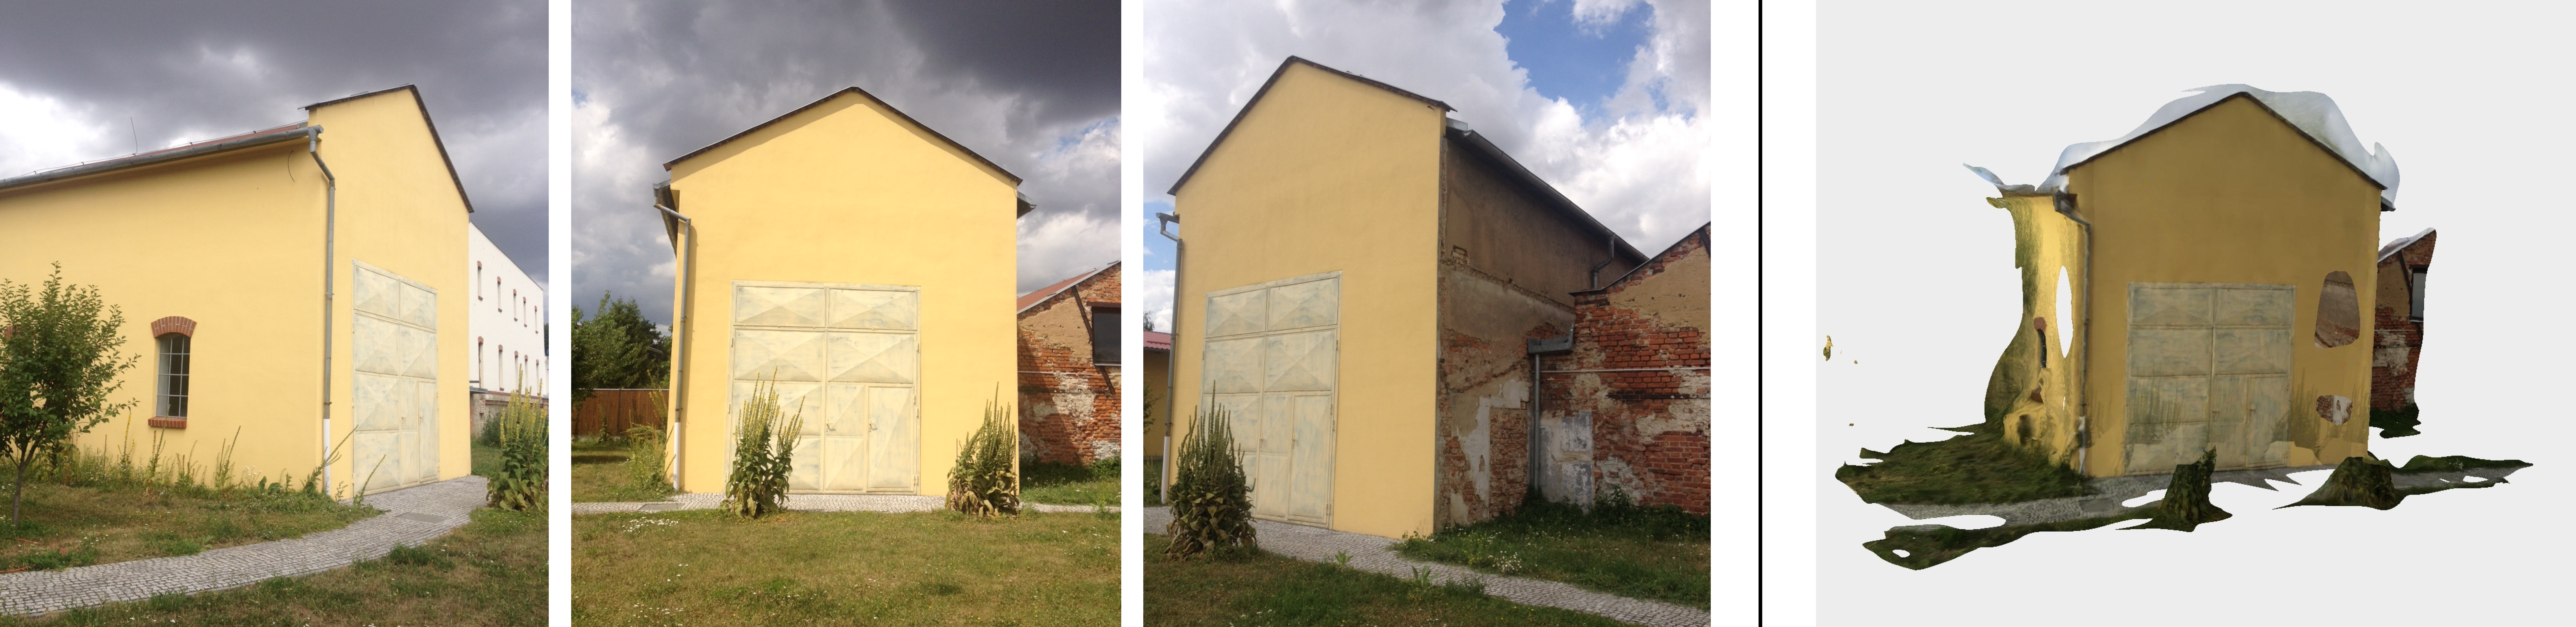
\includegraphics[keepaspectratio,width=\textwidth]{fig/123d.pdf}
	\end{center}
	\caption{3D model (right) obtained from the Autodesk 123D Catch application on iOS.}
	\label{fig:openvmg}
\end{figure}

\subsection*{Sketchup and Blender}
While we are mainly interested in an automated process of creating 3D models from a set of 2D pictures, it is worth mentioning that there are solutions for creating 3D models to match 2D images manually. Both the SketchUp\footnote{3D for Everyone | SketchUp, \url{http://www.sketchup.com}} and Blender offer such functionality. The process\footnote{Match Photo: Modeling from photos | SketchUp Knowledge Base, \url{http://help.sketchup.com/en/article/94920}} is rather simple and consists of mapping the $x, y$ and $z$ axes to the picture and than drawing over it. Once done, next picture is matched and rest of the visible structure drawn. The figure~\ref{fig:sketchup} shows the process of creating a simple 3D model in SketchUp.

\begin{figure}[ht]
	\begin{center}
		\includegraphics[keepaspectratio,width=\textwidth]{fig/sketchup_modelhouse.pdf}
	\end{center}
	\caption{Creating a simple 3D model of the Model House (will be introduced later in section~\ref{sec:experiments-datasets}) in SketchUp.}
	\label{fig:sketchup}
\end{figure}

\subsection*{SLAM\textunderscore frontend and SLAM++}
The SLAM\textunderscore frontend  and SLAM++ developed at the Faculty of Information Technology at Brno University of Technology, are libraries for the bundle adjustment and structure from motion applications. It is worth mentioning, that the SLAM\textunderscore frontend is still under development and so far was not released. The SLAM++ is a library containing several methods used in problems like bundle adjustment, structure from motion, simultaneous localization and mapping (SLAM) and many others. The core of the library is a general graph optimizer along with several problem solvers, nonlinear least squares solvers and block linear solvers. It is written in C++ and it is very fast due to the fact that it exploits the block structure the problems and offers very fast solutions to manipulate block matrices within iterative nonlinear solvers (this will be detailed in the section~\ref{sec:bundle-adjustment}).

The SLAM\textunderscore frontend is a collection of applications that take as input image files or any other sensor data files and generate inputs for the SLAM++ block-sparse linear algebra SLAM solver. Apart form SLAM++, it requires OpenCV. The SLAM\textunderscore frontend is also an easy to use interface for implementing custom structure from motion or bundle adjustment application. It provides means to load set of images and detect, extract and match features. The framework provides templates for custom estimators, such that one can implement camera pose estimator for a BA application. Right now there are three finished applications:

\begin{itemize}
	\item The \textbf{Mono app} which reconstructs 3D scene from an ordered image dataset made by single camera with known intrinsic camera parameters.
	
	\item The \textbf{Spheron app} reconstruct the 3D scene from a spheron camera with known intrinsic camera parameters.
	
	\item The \textbf{Stereo app} uses a stereo vision to reconstruct the 3D scene from a pair of horizontally displaced cameras with known intrinsic camera parameters .
	
	\item Lastly, the \textbf{Uncalibrated app} which attempts to implement the general bundle adjustment problem (unordered image dataset with unknown intrinsic camera calibration). The application is subject of this thesis and the implementation will be further described described in chapter~\ref{chapter:implementation}.
\end{itemize}

\section{Detectors}
\label{sec:detectors}
A successful 3D reconstruction stands and falls on good feature detection. The quality and the robustness of features is usually much more important then their quantity which will be demonstrated later in this section. The ideal feature detector finds salient image regions such that they are repeatedly detected despite change of viewpoint; more generally it is robust to all possible image transformations. Therefore, it does not detect any points in uniform and uninteresting surfaces like sky or texture-less walls. The best detector to be used depends heavily on the requested task. In our application features we are interested in are edges and corners of buildings and their distinct parts.

We can divide types of image features into following categories (please note that a detector can detect features from multiple categories):
\begin{itemize}
	\item \textbf{Edge} is a point where there is a sudden change between adjacent pixels (strong gradient magnitude). Generally an edge can be of almost any arbitrary shape and may include junctions. Locally edges have a one-dimensional structure.
	\item \textbf{Interest point} has a local two dimensional structure. We can think of it as two-dimensional edge, in fact early algorithms were used to detect interest points as edges and then selected the interest points by further calculation. In some literature you the interest points may be referred to as corners.
	\item \textbf{Blobs} provide a complementary description of image structures in terms of regions, as opposed to corners that are more point-like. A term regions of interest or interest points are sometimes used as the blob descriptors often contain a preferred point (a local maximum or a center of gravity). Blobs allows detection of smooth areas in an image that might not be detected as an edge or corner.
	\item \textbf{Ridges} are in computer vision a set of curves whose points are have a local maximum in at least one dimension. This notion captures the intuition of geographical ridges. Ridge detection is usually much harder then Edge, Interest point or Blob detection.
\end{itemize}

The detector algorithms used are implemented in the Open source Computer Vision (OpenCV)\footnote{OpenCV | OpenCV, \url{http://opencv.org}} library but other implementations exist (eg. VLFeat\footnote{A. Vedaldi and B. Fulkerson, VLFeat: An Open and Portable Library of Computer Vision Algorithms, 2008, \url{http://www.vlfeat.org/}}). The OpenCV was designed with a strong focus on real-time applications and contains number of algorithms from computer vision. In the remainder of this section feature detectors wrapped in the SLAM\textunderscore frontend will be presented and briefly compared as we will evaluate their performance for our problem in section~\ref{sec:experiments-extractors}.

	
\begin{itemize}
	\item[1.] The \textbf{Harris Corner Detector} is one of the most known feature detectors . It can identify similar regions between images that are related through affine transformations and have different illuminations. Even though the Harris Corner Detector is fast, it does not select enough keypoints and therefore is not suitable for the 3D building reconstruction\footnote{Harris corner detector - OpenCV 2.4.9.0 documentation, \url{http://docs.opencv.org/doc/tutorials/features2d/trackingmotion/harris_detector/harris_detector.html}}.
	
	\item[2.] The \textbf{Good feature to Track (GFTT)} detector is modified version of the Harris Corner Detector described earlier. It is still classified as a corner detector, however, the scoring function differs. Compared to the Harris, the algorithm was slightly slower, with higher amount of features. Nevertheless, both of these algorithms do not perform well enough for our problem~\cite{article:gftt}.
	
	\item[3.] A \textbf{Scale-invariant feature transform} (or SIFT) is an algorithm in computer vision to detect and describe local features in images. The algorithm was published by David Lowe in 1999. The algorithm uses as a keypoints image structures which resemble blobs. The use of the detector is licensed which is an argument against using of this detector in our application. However, as expected, the detector performs very well and is used in many other SfM and BA tools presented earlier~\cite{article:sift}.
	
	\item[4.] The \textbf{Speeded Up Robust feature (SURF)} detector is modification of the SIFT detector. It addresses the slow processing of the SIFT while maintaining reasonable efficiency. While it can surely be used in the SfM application, from our experiments we discovered that the increased performance greatly decreases feature detection for (in our case) important structures~\cite{surf}.
	
	\item[5.] The \textbf{Feature from Accelerated Segment Test (FAST)} aims to rapidly increase performance of feature detection while sustaining feature quality of SIFT-like detectors. The algorithm detects corners in the image and should be used with SIFT or SURF extractor for best performance. In our case,  the FAST selects three times more features and it is hundred times faster than SIFT (resp. 50 times faster than SURF) we mark this as one of the interesting detectors for the final implementation~\cite{article:fast}.
	
	\item[6.] The \textbf{Robust Invariant Scalable Keypoints (BRISK)} detector uses scale-space pyramid layers of octaves and intra-octaves to detect corners in an image. The algorithm uses FAST feature detector score and was developed to get the better of SIFT and SURF detectors. However, in our case the performance gain is not worth decreased feature quality~\cite{article:brisk}.
	
	\item[7.] \textbf{Dense Sampling} uses a regular grid to find a keypoints in the image. This results in good coverage of the entire object or scene and a constant amount of features per image area. The dense sampling is fast as the detector selects all points on a grid without analysis of the surrounding. On the downside, dense sampling cannot reach the same level of repeatability as obtained with interest points, unless sampling is performed extremely densely, but then the number of features quickly grows unacceptably large. The dense sampling is therefore not useful in the SfM model estimation, but can be used for a dense reconstruction once sparse structure is calculated~\cite{article:dense}.
	
	\item[8] The \textbf{Oriented FAST and Rotated BRIEF (ORB)} detector originated from the OpenCV Labs. Its goal was to offer robustness of a SIFT and SURF, while maintaining fast processing time like FAST and BRIEF combination. While this may be true, for our problem the ORB detector does not perform well enough. The features found rarely belong to a building and usually chunks around trees and vegetation~\cite{article:orb}.
	
	\item[8.] The \textbf{Maximally Stable Extremal Regions} is a blob detector. The MSER algorithm extracts from an image a number of co-variant regions, called MSERs: an MSER is a stable connected component of some gray-level sets of the image. MSER is based on the idea of taking regions which stay nearly the same through a wide range of thresholds~\cite{mser}. For our task this detector performs poorly and takes even more time than SIFT detector.
\end{itemize}

\section{Extractors}
\label{sec:extractors}
In order to work further with the keypoints detected in previous step, the keypoints have to be analysed and transformed into so called feature descriptors (often only the term features or descriptors is used). The process consists of inspecting local image patch around the keypoint to be extracted. This extraction may involve quite considerable amounts of image processing and involves reducing the amount of resources required to describe the original data. The result is known as a feature descriptor or a feature vector. Among the information that may be stored within feature descriptor, one can mention local histograms. In addition to such attribute information, the keypoints detection step may also provide complementary attributes, such as the edge orientation, gradient magnitude in edge detection and the polarity or the strength of the blob in blob detection. The authors of detectors usually specify which extractor should work best for their detection algorithm, some even provide their own.

There are two types of descriptors in OpenCV library; a) descriptors using floating point numbers and b) descriptors storing information as a binary data in unsigned char type.
\begin{itemize}
	\item[a)] \textbf{Float} descriptors:
	
	\begin{itemize}
		\item \textbf{SIFT:} The scale-invariant feature transform of a neighbourhood is a 128-dimensional vector of histograms of image gradients. The region, at the appropriate scale and orientation, is divided into a $4\times 4$ square grid, each cell of which yields a histogram with 8 orientation bins. The SIFT extractor is advised to be used with the SIFT, SURF and FAST detector.
		\item \textbf{SURF:} The speeded up robust feature extractor uses either 128 or 64-dimensional vector of histograms of image gradients.An oriented quadratic grid of $4 \times 4$ square sub-regions is laid over the keypoint and a wavelet response computed for each square. According to literature the SIFT, SURF and FAST detector can be used with the SURF extractor~\cite{surf}.
	\end{itemize}
	
	\item[b)] \textbf{Binary} descriptors:
	
	\begin{itemize}
		\item \textbf{BRIEF:} The Binary Robust Independent Elementary Feature descriptor is a 128, 256 or 512-dimensional bitstring which is a good compromise between speed, storage efficiency and recognition rate. The descriptor is much smaller (16, 32 or 64 bytes) compared to floating point descriptors, while maintaining a good performance compared to SURF or U-SURF~\cite{article:brief}.
		
		\item \textbf{ORB:} Unlike BRIEF, Oriented FAST and Rotated BRIEF (ORB) is comparatively scale and rotation invariant while still employing the very efficient Hamming distance\footnote{University of Manchester, Coding Theory lecture notes, \url{http://www.maths.manchester.ac.uk/~pas/code/notes/part2.pdf}} metric for matching. As such, it is preferred for real-time applications, but may be suitable for some offline applications as well~\cite{article:orb}.
		
		\item \textbf{FREAK:} The Fast Retina Keypoint extractor aims to be faster and more robust than SIFT and SURF extractors. It uses a novel keypoint descriptor inspired by the human visual system to compute cascade of binary strings~\cite{article:freak}.
		
		\item \textbf{BRISK:}  The  Binary Robust Invariant Scalable Keypoints extractor uses a 64-byte binary descriptor composed as a binary string by concatenating the results of simple brightness comparison tests~\cite{article:brisk}.
	\end{itemize}
\end{itemize}

\section{Matchers}
\label{sec:matchers}
So far we are able to find points of interest in an image and describe them in such a way that they are effectively stored but still contain information about the point and its local image patch. Once descriptors are extracted from two or more images, we want to match points present in more then one image. This is effectively a nearest neighbour search~\cite{nearest_neighbour_search} which is an optimization problem for finding closest (or most similar) points. There are two approaches to this problem that are implemented in the OpenCV: a) Brute-Force and b) Approximate Nearest Neighbour (ANN)-based matching.

\begin{itemize}
	\item[a)] The Brute-Force matcher is simple and naive approach. It takes the descriptor of one feature from the first image set and matches it with all other feature from the second image set. During the process a distance of some sort is calculated and the match with best metric selected. There are number of metrics implemented in the OpenCV to be used with different descriptors but we, once again, tried all the combinations in order to get best result for our problem. The algorithm promises best possible matches, but due to the fact that it tries to match each pair of features, can take a lot of time to process. 

	\item[b)] The Fast Library for Approximate Nearest Neighbors (FLANN) implemented in OpenCV, performs a fast ANN searches in high dimensional spaces. It uses the Hierachical K-means Tree for generic feature matching. Nearest neighbors are discovered by choosing to examine the branch-not-taken nodes along the way~\cite{flann}.
\end{itemize}

\chapter{Methodology}
\label{chapter:methodology}
\textit{This chapter thoroughly describes the whole 3D reconstruction process. First, the general pipeline is outlined and each step briefly discussed. Second, the camera model is presented. The reader will learn about the intrinsic and extrinsic camera parameters, distortion and how does it relate to the camera pose. Next we talk about the epipolar geometry and fundamental matrix which allows us to obtain the camera poses and reconstruct the scene up to some degree of ambiguity. The main focus of the chapter is on the 3D reconstruction. We start with the 3D reconstruction approaches and what form of reconstruction can be achieved in various scenarios. The chapter continues with the stereoscopic and multiple-view camera calibration and finishes of with bundle adjustment. That is the refinement of estimated 3D model and camera calibrations.}

\begin{figure}[t]
	\begin{center}
		\includegraphics[keepaspectratio,width=\textwidth]{fig/pipeline.pdf}
	\end{center}
	\caption{The three-dimensional structure from two-dimensional images estimation pipeline to be implemented in the final application.}
	\label{fig:pipeline}
\end{figure}

\section{Three-dimensional Structure Estimation Pipeline}
\label{sec:pipeline}
The pipeline of the 3D reconstruction application (depicted in figure~\ref{fig:pipeline}) consists of 7 distinct steps:
\begin{itemize}
	\item[1.] \textbf{Dataset aquisition.} First step in the 3D reconstruction pipeline is the selection of input data. Specific requirements on the data varies throughout different software, however, we can generalize some properties of such set of images. The set has to contain images that are overlapping one another, depict mostly static scene, are not too general (for example an image sequence along one face of a building with multiple similarly looking windows) and contain little to none reflection. Only such images are used in the reconstruction as they provide points seen by multiple cameras and therefore the 3D position can be calculated.
	\item[2.] \textbf{Feature detection and extraction.} Keypoints are parts of the image that are significant in some way. The significance is usually caused by a sudden change in gradient on relatively small part of the image. These points will be used to estimate the 3D representation. The detected keypoints are rarely used as provided by the detector as they do not provide enough information about the point itself. A set of calculations is applied in order to extract data from the surroundings of such point and enrich information about the keypoint. At this point the input image does not have to be kept in memory any more.
	\item[3.] \textbf{Feature matching.} Now that we have keypoints represented as features we want to establish a visual correspondence between a set of keypoints from two closely related images. This is done by so called feature matching and was discussed in detail in section~\ref{sec:matchers}.
	\item[4.] \textbf{Features and camera track building.} The problem of features tracking is to follow the position of a characteristic point in a set of images. These multi-view correspondences are called tracks. Track identification in a set of images (ordered, or not) is an important task in not only our application but in many other computer vision problems. Another part of this problem is building camera tracks - estimating sequences or bunches of cameras which together form a model and selecting initial camera pair.
	\item[5.] \textbf{Camera pose estimation.} Once correspondence between some two images are known, the camera pose can be estimate. This can be divided into two cases: 1) this is first camera pair in the scene (initialization) 2) there are already some cameras and structure points in scene, and the new camera pose can be estimated from 2D - 3D correspondences.
	\item[6.] \textbf{Structure computation.} Next step is to calculate 3D structure from camera poses obtained earlier. This is also incremental process which consist of initialization for the first camera pair and addition of new structure points to an existing structure for each newly added camera.
	\item[7.] \textbf{Structure refinement.} The structure and camera poses in the scene are subject to errors caused by reprojection ambiguity, distortion etc. Therefore the structure needs to be refined to minimize the impact of such errors.
	\item[8.] \textbf{Visualization and further processing.} Lastly the resulting 3D structure in form of point cloud is visualized. In this thesis we will not be interested in the visualization of the resulting model, however we see this as an important part of the bundle adjustment pipeline. As of now there are no plans to implement visualization of a final sparse reconstruction, but the output of our application is a 3D point cloud with camera poses in a PLY format that can be displayed in many 3D editing applications (eg. Blender introduced earlier). There are also means to further process the output in order to create a polygonal model (either manually using programs like MeshLab, Blender, SketchUp or automatically using programs and libraries; eg. Point Cloud Library~\cite{PCL} or PMVS and CMVS mentioned earlier). 
\end{itemize}

\section{Camera Model}
Before we explain the reconstruction process, it is important to explain how is the camera modelled. For purpose of this thesis we will be using the pin-hole camera model (or sometimes projective camera model) which is a widely used in many computer vision applications. It is simple and accurate enough for most applications. The name comes from the type of camera, like a camera obscura, that collects light through a small hole to the inside of a dark box or room. In the pin-hole camera model, light passes through a single point, the camera center $C$ before it is projected onto an image plane. Figure~\ref{fig:cameramodel} shows an illustration where the image plane is drawn in front of the camera center. The image plane in an actual camera would be upside down behind the camera center, but the model is the same.

\begin{figure}[ht]
	\begin{center}
		\includegraphics[keepaspectratio,width=\textwidth]{fig/camera-model.pdf}
	\end{center}
	\caption{The pin-hole camera model showing projection of 3D point $M$ on the image plane as a 2D point $m$. An oriented central projective camera.}
	\label{fig:cameramodel}
\end{figure}

The projection properties of a pin-hole camera can be derived from this illustration and the assumption that the image axis is aligned with the $X$ and $Y$ axis of a 3D coordinate system. The optical axis of the camera then coincides with the z axis and the projection follows from similar triangles. By adding rotation and translation to put a 3D point in this coordinate system before projecting, the complete projection transform follows.

With a pin-hole camera, a 3D point $M$ is projected to an image point $m$ (both expressed in homogeneous coordinates) as:

\begin{equation}
  \begin{aligned}
	\lambda m&= PM \\
	\lambda
	\begin{pmatrix}
		x \\
		y \\
		1 \\
	\end{pmatrix}
	&=
	\begin{bmatrix}
		p_{1,1} & p_{1,2} & p_{1,3}  & p_{1,4} \\
		p_{2,1} & p_{2,2} & p_{2,3}  & p_{2,4} \\
		p_{3,1} & p_{3,2} & p_{3,3}  & p_{3,4} \\
	\end{bmatrix}
	\begin{pmatrix}
		X \\
		Y \\
		Z \\
		1 \\
	\end{pmatrix},
	\end{aligned}
	\label{eq:point-projection}
\end{equation}
where $\lambda$ is the distance of $M$ from the focal plane of the camera. The projection matrix $P$ is a $3 \times 4$ matrix defined as:
\begin{equation}
	P_{3 \times 4}= K_{3 \times 3}A_{3 \times 4},
\end{equation}
where $K$ is intrinsic camera matrix which describes some of the properties of the physical camera and represents 2D transformation on the image plane. The camera matrix have 5 degrees of freedom (DOF). We write:
\begin{equation}
	K_{3 \times 3} = 
	\begin{bmatrix}
		f/s_x & f/s_x  cot \phi & c_x \\
		0 & f/s_y & c_y \\
		0 & 0  & 1 \\
	\end{bmatrix},
\end{equation}
where $f$ is the camera focal distance in millimeters, $c_x, c_y$ are coordinates of camera's principal point (image centre) in pixels, $s_x$ resp $s_y$ is width resp height of the pixel footprint on the camera photosensor in millimeters and $\phi$ is the angle between the axis (usually $\pi /2$). The ratio $s_y/s_x$ is called aspect ratio and is usually close to 1.

Matrix $A$ then refers to the extrinsic camera parameters and describes the camera position(3 DOF) and rotation (3 DOF) on the 3D coordinate system (see figure~\ref{fig:cameramodel}).

\begin{equation}
	A_{3 \times 4} = [R_{3 \times 3} |t_{1 \times 3}] =
	\begin{bmatrix}[ccc|c]
		r_{1,1} & r_{1,2} & r_{1,3} & t_{x} \\
		r_{2,1} & r_{2,2} & r_{2,3} & t_{y} \\
		r_{3,1} & r_{3,2} & r_{3,3} & t_{z} \\
	\end{bmatrix}
\end{equation}
This matrix describes how to transform points in world coordinates to camera coordinates. The vector $t$ can be interpreted as the position of the world origin in camera coordinates, and the columns of $R$ represent the directions of the world-axes in camera coordinates. The important thing to remember about the extrinsic matrix is that it describes how the world is transformed relative to the camera~\cite{solem}.

\begin{figure}[!htbp]
	\begin{center}
		\includegraphics[keepaspectratio,width=\textwidth]{fig/distortion.pdf}
	\end{center}
	\caption{Illustration of radial distortion effect.}
	\label{fig:dist}
\end{figure}

The previously described model is an ideal camera without any lens distortion. However, real cameras suffer from distortion. The most common distortion is a radial distortion (depicted in figure~\ref{fig:dist}) that can be characterized by following equation (distortion around $(0,0)$):
\begin{equation}
	\begin{bmatrix}
		x_{dist} \\
		y_{dist} \\
	\end{bmatrix}
	= (1 + k_1(x^2_{undist}, y^2_{undist}) + k_2(x^2_{undist}, y^2_{undist})^2)
	\begin{bmatrix}
		x_{undist} \\
		y_{undist} \\
	\end{bmatrix},
	\label{distortion}
\end{equation}
where $k_1,k_2$ are distortion parameters. In our program will only model radial distortion.

\section{Epipolar Geometry}
Lets have a scene where either: 1) scene is static and camera moves, or 2) there are multiple pictures of same scene taken at the exactly same time from different viewpoints, which is ultimately the same as case 1. Given two distinct images of the scene taken from different positions we can re-project a point (for example a detected feature) from one camera into the 3D space. Because the point has one degree of freedom, it can be observed somewhere on a line in the second camera. And similarly a point in second camera is projected somewhere on a line in the first camera. These lines are called the epipolar lines. A line connecting centres of both cameras is called baseline and the intersection with the image plane the epipole. All epipolar lines in each image intersect in the epipole. The corresponding epipolar lines from camera 1 and camera 2 (conjugate epipolar lines) constrain the search of correspondences~\cite{book:multiple_view_geometry}.

\begin{figure}[!htbp]
	\begin{center}
		\includegraphics[keepaspectratio,width=\textwidth]{fig/epipolar-lines.pdf}
	\end{center}
	\caption{An illustration of epipolar line in camera 2 for point $m$ in camera 1.}
	\label{fig:epipolar-lines}
\end{figure}

\begin{figure}[!htbp]
	\begin{center}
		\includegraphics[keepaspectratio,width=\textwidth]{fig/epipolar-lines2.pdf}
	\end{center}
	\caption{An illustration of constraint given by epipolar lines to the search of correspondence problem (the red and blue lines in each image are in pairs conjugate epipolar lines).}
	\label{fig:epipolar-lines2}
\end{figure}

The epipolar lines can be obtain from a fundamental matrix. The fundamental matrix $F$ is a $3 \times 3$ matrix defined as:
\begin{equation}
	\begin{bmatrix}
		x_1 & y_1 & 1 \\
	\end{bmatrix}
	F
	\begin{bmatrix}
		x_2 \\
		y_2 \\
		1 \\
	\end{bmatrix}
	= 0
	\label{eq:fundamental-matrix}
\end{equation}
for any $(x_1, y_1) \leftrightarrow (x_2, y_2)$ correspondence, $(x_1, y_1)$ in image 1 and $(x_2, y_2)$ in image 2. If we fix the $(x_2, y_2)$ we get an epipolar line for the first image by:
\begin{equation}
	\begin{bmatrix}
		x_1 & y_1 & 1 \\
	\end{bmatrix}
	F
	\begin{bmatrix}
		x_2 \\
		y_2 \\
		1 \\
	\end{bmatrix}
	=
	\begin{bmatrix}
		x_1 & y_1 & 1 \\
	\end{bmatrix}
	\begin{bmatrix}
		a \\
		b \\
		c \\
	\end{bmatrix}
	= 0,
\end{equation}
which gives us the epipolar line equation
\begin{equation}
	ax_1 + by_1 + c = 0.
\end{equation}

Even though the fundamental matrix is a $3 \times 3$ matrix, it only has 7 degrees of freedom (one constraint is scale second is the existence of epipole, the derivation can be found in~\cite{book:multiple_view_geometry}). Now that we know the characteristics of the fundamental matrix we can estimate it using several algorithms, following is the eight-point algorithm~\cite{cvfx, elements-of-computer-vision, book:multiple_view_geometry} (requires at least 8 correspondences):
\begin{itemize}
	\item[1.] Obtain feature correspondences 
	\item[2.] Normalize correspondence to have standard deviation=1 and mean=0
	\item[3.] Given $n$ correspondences, $n \geq 8$, create an equation for each correspondence $i, 1 \leq i \leq n$:
	\begin{equation}
		m_{i_1} F m_{i_2} = 
		\begin{bmatrix}
			x_{i_1} & y_{i_1} & 1 \\
		\end{bmatrix}
		\begin{bmatrix}
			f_{1,1} & f_{1,2} & f_{1,3} \\
			f_{2,1} & f_{2,2} & f_{2,3} \\
			f_{3,1} & f_{3,2} & f_{3,3} \\
		\end{bmatrix}
		\begin{bmatrix}
			x_{i_2} \\
			y_{i_2} \\
			1 \\
		\end{bmatrix}
		= 0
	\end{equation}
	and create the system:
	\begin{equation}
		A_{n \times 9}F_{1 \times 9}=
		\begin{bmatrix}
			x_{1_1} x_{1_2} & x_{1_1} y_{1_2}  & x_{1_1}  & y_{1_1} x_{1_2} & y_{1_1} y_{1_2}  & y_{1_1}  & x_{1_2} & y_{1_2}  & 1 \\
			. & . & . & . & . & . & . & . & .\\
			. & . & . & . & . & . & . & . & .\\
			. & . & . & . & . & . & . & . & .\\
			x_{n_1} x_{n_2} & x_{n_1} y_{n_2}  & x_{n_1}  & y_{n_1} x_{n_2} & y_{n_1} y_{n_2}  & y_{n_1}  & x_{n_2} & y_{n_2}  & 1 \\
		\end{bmatrix}
		\begin{bmatrix}
			f_{1,1} \\
			f_{1,2} \\
			. \\
			. \\
			. \\
			f_{3,3} \\
		\end{bmatrix}
		= 0
	\end{equation}
	\item[4.] Compute singular value decomposition of A
		\begin{equation}
			A = UDV^T
		\end{equation}
	\item[5.] Let $F$ be the last column of $V$ and reshape $F$ to be  $F'_{3 \times 3}$.
	\item[6.] Compute SVD of $F'=U'D'V'^T$, zero out the lowest singular value of $D'$ then recompute $F = U'D'V'^T$
	\item[7.] Re-normalize $F$
\end{itemize}
There are several other methods which require less points or have other benefits. Interested reader may find the whole list in~\cite{book:multiple_view_geometry}.

\section{Stereo and Multi-view Stereo Camera Calibration}
The epipolar geometry can be described analytically in several ways, depending on the amount of the knowledge about the system. We can identify three general cases:
\begin{itemize}
	\item[1.] Neither intrinsic nor extrinsic camera parameters are known, the epipolar geometry is described by fundamental matrix. This is called projective reconstruction and the only information available are pixel correspondences. The reconstruction problem can be solved but only up to an unknown, global projective transformation of the world.  By providing other restrictions on the model we can reduce the ambiguity.
	\item[2.] Only intrinsic camera parameters are known, the epipolar geometry is described by the essential matrix. The reconstruction is ambiguous up to scale and a rigid transformation corresponding to the freedom in fixing the world reference frame - reconstruction up to a similarity called euclidean or metric.
	\item[3.] Both intrinsic and extrinsic camera parameters are known, the epipolar geometry is described by the projection matrices. The reconstruction is unambiguous. This case will not be further discussed as this is not the goal of this thesis.
\end{itemize}

\begin{figure}[ht]
	\begin{center}
		\includegraphics[keepaspectratio,width=\textwidth]{fig/stereo2.pdf}
	\end{center}
	\caption{Illustration of stereo system camera for camera calibration.}
	\label{fig:stereo2}
\end{figure}

The goal of the pose estimation is to, given two cameras, estimate their calibration matrices $P_1$ and $P_2$. Let there be a system with two cameras pointing at the same object with enough 3D points visible in both cameras~\ref{fig:stereo2}. 
\subsection*{1. Projective Reconstruction}
We start with the most general case, the projective reconstruction. First we need to calculate the fundamental matrix $F$ between these two cameras which gives us the transformation between points in both images, described by equation~\ref{eq:fundamental-matrix}. Let
\begin{equation}
	P_1= K_1[I|0] =
	\begin{bmatrix}
		f/s_x & f/s_x  cot \phi & c_x \\
		0 & f/s_y & c_y \\
		0 & 0  & 1 \\
	\end{bmatrix}
	\begin{bmatrix}[ccc|c]
		1 & 0 & 0 & 0 \\
		0 & 1 & 0 & 0 \\
		0 & 0 & 1 & 0 \\
	\end{bmatrix}
\end{equation}
be the first camera matrix. Then we search for the
\begin{equation}
	P_2 = K_2[R|t]. 
\end{equation}
Now we can easily calculate the epipoles $e_1, e_2$ as:
\begin{equation}
  \begin{aligned}
	e_1 &\sim P(-R^T t) = K_1 [I|0]
	\begin{bmatrix}
		-R^T t \\
		1 \\
	\end{bmatrix} \sim K_1 R^Tt \\
	e_2 &\sim K_2[R|t]
	\begin{bmatrix}
		0 \\
		0 \\
		0 \\
		1 \\
	\end{bmatrix} \sim K_2 t.
  \end{aligned}
\end{equation}
If the intrinsic camera parameters are unknown, the projection matrix $P_2$ can be estimated using epipolar lines:
\begin{equation}
	P_2 = 
	\begin{bmatrix}
		\begin{bmatrix}
			e_2 \\ 
		\end{bmatrix}_{\times} F + e_2 v^T | \lambda e_2 \\
	\end{bmatrix}
\end{equation}
where $v$ is a $3 \times 1$ vector and $\lambda$ any non-zero scalar value. 
\subsection*{2. Euclidean reconstruction}
However, if the intrinsic camera matrices $K_1, K_2$ are known, we can transform the corresponding points.
\begin{equation}
  \begin{aligned}
	m'_1 &= K_1^{-1} m_1 \\
	m'_2 &= K_2^{-1} m_2
  \end{aligned}
	\label{eq:calib-x}
\end{equation}
Then the camera matrices can be written in form:
\begin{equation}
  \begin{aligned}
	P_1 &= [I|0] \\
	P_2 &= [R|t] 
  \end{aligned}
\end{equation}
The fundamental matrix can now be either recalculated from transformed correspondences given by equation~\ref{eq:calib-x} or modified using the calibration matrices into special form called the essential matrix $E$.
\begin{equation}
	E = K_1^{-T} F K_2^{-1}
\end{equation}
The rotation matrix $R$ and translation vector $t$ is then obtained by a singular value decomposition of $F = UDV^T$ which gives us four options:
\begin{equation}
  \begin{aligned}
	P_2 &= \{[UWV^T | \pm u_3], [UW^T V^T | \pm u_3]\} \\
	W &= 
	\begin{bmatrix}
		0 & -1 & 0 \\	
		1 & 0 & 0 \\	
		0 & 0 & 1 \\	
	\end{bmatrix}
  \end{aligned}
\end{equation}
\begin{figure}[!htbp]
	\begin{center}
		\includegraphics[keepaspectratio,width=\textwidth]{fig/calibration-options.pdf}
	\end{center}
	\caption{Four possible options of camera calibration when the intrinsic camera parameters are known.}
	\label{fig:caliboptions}
\end{figure}
where $u_3$ is the last column of $U$. By triangulation (described in next section) we can resolve which of these four options is the correct one (selected 3D point is in front of the camera as shown in figure~\ref{fig:caliboptions} a))~\cite{cvfx, elements-of-computer-vision, book:multiple_view_geometry}.

\section{Three-dimensional Reconstruction Approaches}
Based on the image source we can distinguish between three types of vision: stereoscopic, monocular and uncalibrated. The type of the vision defines the difficulty of the 3D reconstruction problem~\cite{book:multiple_view_geometry}.

\begin{figure}[ht]
	\begin{center}
		\includegraphics[keepaspectratio,width=\textwidth]{fig/stereo.pdf}
	\end{center}
	\caption{An illustration of obtaining the 3D position from stereo image.}
	\label{fig:stereo}
\end{figure}

\subsection*{Stereoscopic Vision}
The stereoscopic vision is similar to human binocular vision. Two cameras, displaced horizontally from one another are used to obtain view of the scene, simulating human vision. By comparing both images, the relative depth information can be obtained, which is proportional to the differences in distance to the objects. If the images are undistorted, and camera parameters known, we can easily calculate the 3D relative position of the points. Figure~\ref{fig:stereo} shows how the point 3D position can be calculated using following equations:

\begin{equation}
	\begin{aligned}
		Z&=\frac{f b}{x_1 - x_2 + f* tan(\theta)} \\
		X&= x_1 \frac{Z}{f} \\
		Y&= y_1 \frac{Z}{f} + tan(\phi)Z, \\
	\end{aligned}
\end{equation}
where $\theta$ is a rotation around $Y$ axis and $\phi$ is a rotation around $X$ axis. The rotation ($\psi$) around $Z$ axis is usually dealt with by rotating the image before triangulation. If the cameras are not aligned and the optical axes are not parallel, the 3D coordinates can still be calculated. We present one of the simplest methods called linear transformation, but many other can be find in literature~\cite{Hartley96triangulation, book:multiple_view_geometry}. The overall algorithm for linear transformation requires camera poses and is following:
\begin{itemize}
	\item[1.] Create matrix $A$:
	\begin{equation}
		A = 
		\begin{bmatrix}
			x_1 P_1^T(3) - P_1^T(1) \\
			y_1 P_1^T(3) - P_1^T(2) \\
			x_2 P_2^{T}(2) - P_2^{T}(1) \\
			y_2 P_2^{T}(3) - P_2^{T}(2) \\
		\end{bmatrix},
	\end{equation}
	where the matrix $P$ is represented by the block form: $P = [P(1:3)|P(4)]$ (the bracket denotes a range of columns).
	\item[2.] Compute the singular value decomposition of  $X = AV$.
	\item[3.] The 3D point $M$ in homogeneous coordinates is then $M = X_3$.
\end{itemize}

\begin{figure}[ht]
	\begin{center}
		\includegraphics[keepaspectratio,width=\textwidth]{fig/mono.pdf}
	\end{center}
	\caption{An illustration of the process of camera pose estimation using P3P algorithm.\protect\footnotemark}
	\label{fig:mono}
\end{figure}
\footnotetext{Original image from the Monocular camera 3D reconstruction presentation by Ing. Marek Šolony.}

\subsection*{Monocular Vision}
The monocular vision consists of one camera moving in space. Because we have only one camera, the 3D structure can not be easily calculated as in the aligned stereoscopic vision. Instead the camera poses has to be estimated first (this process is often referred to as a camera calibration). First step is detection of the features in each image and finding feature correspondences. Next, the camera poses are estimated. This consists of two parts: 1) first camera pair pose estimation and 2) additional camera poses estimation. The first camera pair pose estimation was described in the previous section. The next step is triangulation of the feature correspondences from the pair to get the initial 3D structure. Any additional cameras' poses can now be estimated from the 3D structure and the corresponding 2D points. This is known as Perspective-n-Point (PnP) camera pose determination problem and there exist number of different algorithms how to solve it~\cite{Alismail_2011_6990}. In our program we will be using variation of the P3P algorithm which requires at least three 3D $\leftrightarrow$ 2D correspondences. The core of the problem is forming a set of equations:
\begin{equation}
	d_{i,j}^2 = S_i^2 + S_j^2 - 2S_i S_j cos \phi_{i,j}, \text{ for } i,j \in \{(1,2),(1,3),(2,3)\},
\end{equation}
where the $S_i = ||M_i-C||$ is the unknown depth of point $i$ from the camera center in the camera frame, $d_{i,j} = ||M_i-M_j||$ is the known inter-point distance  and the $\phi_{i,j}$ is the angle between each pair of rays and can be calculated from intrinsic camera matrix $K$. 

\begin{figure}[ht]
	\begin{center}
		\includegraphics[keepaspectratio,width=\textwidth]{fig/p3p.pdf}
	\end{center}
	\caption{Canonical depiction of the P3P problem.}
	\label{fig:p3p}
\end{figure}

\subsection*{Uncalibrated Vision}
Until this point the intrinsic camera parameters were shared among all cameras and often known. However, this is not the case when dealing with images downloaded from the internet. Therefore we need to estimate the intrinsic camera parameters first. This process is called autocalibration and there are two classes of methods: 1) direct which solve the intrinsic parameters directly and 2) stratified in which the projective reconstruction is obtained first and then transformed into euclidean reconstruction. Several autocalibration methods can be found in~\cite{book:multiple_view_geometry}. Once the calibration matrices are known, we can continue with the steps described in the monocular vision.

\section{Bundle Adjustment}
\label{sec:bundle-adjustment}
The bundle adjustment is an optimization problem which tries to simultaneously refine 3D coordinates describing the scene geometry as well as the parameters of the camera. It is expressed as a sum of squares of a number of non-linear real-valued functions. Thus, the minimization is achieved using non-linear least squares algorithm. To begin, assume that $n$ 3D points are seen in $k$ views and let $m_{i,j}$ be the projection of the $i$-th point on image $j$. Each camera $j$ is parametrized by a vector $a_j$ (containing the extrinsic and often intrinsic camera parameters) and each 3D point $i$ by a vector $b_j$. For simplicity we assume that all points are visible in all images. The bundle adjustment minimizes the reprojection error with respect to all 3D point and camera parameters:
\begin{equation}
	\underset{a_j b_i}{\min} \overset{n}{\underset{i=1}{\sum}} \overset{k}{\underset{j=1}{\sum}} d(Q(a_j, b_i) ,m_{i,j})^2,
	\label{eq:bundle-adjustment}
\end{equation}
where $Q(a_j, b_i)$ is the predicted projection of point $i$ on image $j$ and $d(x,y)$ denotes the Euclidean distance between the inhomogenous image points represented by $x$ and $y$. Note that if $o$ is the dimension of each $a_j$ and $p$ the dimension of $b_i$ the total number of minimization parameters is $ko + np$. 

The bundle adjustment can be cast as a non-linear minimization problem as follows. A parameter vector 
\begin{equation}
P=(a_1^T,...,a_k^T,...,b_1^T,...,b_n^T)^T
\end{equation}
 is defined by all parameters describing the $k$ projection matrices and the $n$ 3D points. A measurement vector 
 \begin{equation}
 X = (m_{1,1}^T,...,m_{1,k}^T, m_{2,1}^T,...,m_{2,k}^T, m_{n,1}^T,...,m_{n,k}^T)^T
 \end{equation}
 is made up of the measured image point coordinates across all cameras. Let $P_0$ be an initial parameter estimate and $\Sigma_X$ the covarience matrix corresponding to the measured vector $X$ (if not enough information about the system is known, it is an identity matrix). For each parameter vector, an estimated measurement vector 
 \begin{equation}
 	\hat{X} = (\hat{m}_{1,1}^T,...,\hat{m}_{1,k}^T, \hat{m}_{2,1}^T,...,\hat{m}_{2,k}^T, \hat{m}_{n,1}^T,...,\hat{m}_{n,k}^T)^T
 \end{equation}
 with $\hat{m}_{i,j} = Q(a_j,b_i)$. Therefore the bundle adjustment is a minimization of the squared Mahalanobis distance $(X-\hat{X)})^T\Sigma_X^{-1}(X-\hat{X)})$ over $P$~\cite{Lourakis04thedesign}. The complexity of this problem can by improved greatly by exploiting the sparsity of the problem; however, this is beyond the scope of this thesis and interested reader is referred to~\cite{nlsq}.
 
In case with known intrinsic camera parameters, the system we want to solve has for each camera 6 degrees of freedom (3 for rotation and 3 for translation). If the intrinsic parameters are unknown the problem has at least 9 DOF (3 rotation, 3 translation and assuming the pixels are square 3 for intrinsic, up to 6).

\chapter{Implementation}
\label{chapter:implementation}
\textit{This chapter describes the implementation of the 3D reconstruction pipeline outlined in previous chapter. More than on the implementation details, we will focus on the overall design and customization capabilities. The chapter starts with our approach on automated generation of datasets from internet sources. We also provide a means to create datasets from pictures taken by the user and we use the OpenCV calibration library to get the intrinsic camera calibration. Because this application will be included in the SLAM\textunderscore frontend and at some point released for the general public, the section~\ref{sec:implementation-core} presents the key data structures, algorithms and overall pipeline. The thesis finishes with the outline on further processing of the resulting point cloud and camera poses.}

\section{Dataset Generation and Camera Calibration}
\label{sec:camera_calib}
Creating a dataset is a crucial part of the process of estimating three-dimensional structures from two-dimensional image sequences. The dataset has to contain enough images with a feature pairs to be viable for reconstruction. We also want to filter out images taken during the night or throughout various seasons as the depicted object and its surroundings may change significantly. Another problems are too generic photos and photos with reflection, which may degenerate the reconstruction (an example of this phenomenon is in figure~\ref{fig:degenerated-dataset}). The last problem, unique to the datasets from unknown sources, is an existence of a watermark, text or other 2D manipulation of these pictures.

With this in mind we have decided to download images from Flickr webpage. Flickr\footnote{Flickr, a Yahoo company $|$ Flickr - Photo Sharing! \url{https://www.flickr.com}} is well known and widely used web service for sharing pictures. The advantage of this service, in comparison to other picture sharing websites, is the ability to tag the photo. Each image can contain a number of tags describing it. Most of the pictures uploaded contain information about the place where the photo was taken and can be aggregated by that tag. A tool we designed, Flickr downloader\footnote{Flickr downloader \url{https://github.com/xsimet00/Flickr-downloader}}, allows downloading images with specified tag from Flickr in batches. It is an easy to use Python script expecting two parameters; number of photos to be downloaded and a tag to be browsed. The script connects to the Flickr webpage, downloads the search results page, cyclically opens each photo page and downloads the image. The downloaded images are stored to the \texttt{downloaded} output folder.

While the Flickr yields good results for well known places in countries like USA or western Europe, there is not enough images in the Czech Republic yet. This is the reason why we have, for now, decided to use different services, like Google Image\footnote{Google Image search engine \url{https://images.google.com}} search, as well. A second script that works similarly to the Flicker downloader was designed which downloads images from the Google Image search. It is worth noting that such datasets may contain photos subject to copyright. The datasets acquired were manually filtered to eliminate irrelevant images, limit the selection to daytime photos taken in summer.

\begin{figure}[ht]
	\begin{center}
		\includegraphics[keepaspectratio,width=\textwidth]{fig/degenerated-dataset.pdf}
	\end{center}
	\caption{An example of a degenerated reconstruction as a result of too generic photos of the building. Even though there was 7 (out of 40)  photos of the whole building (as illustrated on the left), from any other position the photos could contain at most distance between 2 windows. The resulting reconstruction (on the right) is therefore degenerated and contains only one column of windows instead of four (reconstructed using the Autodesk 123D Catch iOS client).}
	\label{fig:degenerated-dataset}
\end{figure}

However, sometimes a user may find it useful to use a dataset containing pictures he/she has taken. It is likely, that such collection of photos was taken by a single camera and this camera can be further used. Even though the ultimate goal of our program is to process photos from different cameras and estimate their calibration, the reconstruction process is much faster and more precise if the intrinsic camera parameters are known. For this purpose we have used the OpenCV calibration sample, that given at least three images of calibration pattern, calculates the intrinsic camera parameters as well as radial distortion coefficients of the image. The datasets used will be detailed in section~\ref{sec:experiments-datasets}.

\section{Core of the Application}
\label{sec:implementation-core}
The implemented application is part of the SLAM\textunderscore frontend framework and uses many of the classes and functions provided along with the SLAM++ optimizer. The application implements the pipeline introduced earlier starting from step 2, feature detection, and ending with the step 7, optimization of the estimated 3D structure and camera poses. The core of the application is a data structure \texttt{ModelSystem} which encapsulates the information about cameras, feature correspondences, 3D structure and operations on top of them. 
\begin{itemize}
	\item[a.] \textbf{Cameras.} Each camera is described by its intrinsic camera parameters (matrix $K$), extrinsic camera parameters (matrix $[R|t]$), normalized, distorted coordinates of the keypoints in the image (list of $(x, y)$ pixel coordinates with $(0,0)$ at the principal point), radial distortion coefficients and filename of the image. Because the whole system is iterative, new cameras are added to the system gradually and stored in a linear container. The camera structure also provides number of additional information that are used once the system is passed into the optimizer (like IDs of the vertices).
	\item[b.] \textbf{Feature correspondences.} In order to build camera tracks and select initial pair of cameras, we need to store and process how many feature correspondences (from now on referred as matches) there are between every image pair. Once such information is known a list of camera pairs, starting with the initial pair, can be created. Each new pair adds to the scene either one new camera or just new observations of the structure points as a result of newly known relation between two cameras already present in the system. The selection of the initial pair and creation of such list will be described later. For now it is worth noting that the matrix of such camera pairs is symmetric and sparse as many cameras probably do not share any matches. An illustration of such matrix for real dataset is in figure~\ref{fig:matches-matrix}.
	\item[c.] \textbf{Structure points.} The last important data structure is a collection of the structure points. The problem we are facing here, is the tracking of the 3D point observed by several cameras as some 2D keypoint. Therefore, the structure point is in our system described by its 3D coordinate, list of observations representing the feature track (pairs camera ID, keypoint ID), vertex ID in the optimizer and several flags indicating whether the 3D point is valid and if it needs to be optimized.
\end{itemize}

\begin{figure}[htb]
	\begin{center}
		\includegraphics[keepaspectratio,width=12cm]{fig/matches-matrix.pdf}
	\end{center}
	\caption{The matrix of matches showing number of feature correspondences between each two images for the Guilford Cathedral dataset (described in section~\ref{sec:experiments-datasets}). Each column and row in the matrix represents some image, and the darker the color of the cell is, the more feature correspondences there is for given image pair. It is a square shaped, sparse and diagonally symmetric matrix. }
	\label{fig:matches-matrix}
\end{figure}


Now that the reader is familiar with the key data structures, we can continue explaining the rest of the pipeline from section~\ref{sec:pipeline}. The core of the pipeline is in the method \texttt{run()} in the \texttt{UncalibratedProcessingLoop} class.

\begin{itemize}
\item[\textbf{2.}] \textbf{Keypoints Detection and Feature Extraction.}
So at this point we have an input dataset of photos (and possibly intrinsic camera parameters). The next step in the pipeline is keypoint detection and extraction of the feature descriptors. The \texttt{UncalibratedProcessingLoop} class is effectively a template taking the type of the feature detector as a template parameter. This allows us, with little to none overhead, change the type of detector and extractor. Because not all of the detectors described earlier are build in the SLAM\textunderscore frontend, an interface between the SLAM\textunderscore frontend and the OpenCV was created. The interface is again a \texttt{C++} template. The distinct extractors are defined using the \texttt{typedef} keyword and naming convention follows this scheme: \texttt{FeatureExtractor\textunderscore OpenCV\textunderscore[detector]\textunderscore[extractor]} (eg. \texttt{FeatureExtractor\textunderscore OpenCV\textunderscore SIFT\textunderscore SIFT}). The detected keypoints are stored in the camera class described earlier, but because the feature descriptors are only needed for matching, they can be inserted to a temporal list and cleared later.

\item[\textbf{3.}] \textbf{Feature Matching.}
After extracting features from each image we need to determine which keypoints from distinct images represent the same structure point. These correspondences will be obtained using the FLANN matcher (but again one can provide different matcher as a template parameter). The matches are then filtered to remove outliers and, if enough matches persist, stored in the matrix of matches. At this point it is worth discussing the impact of ordered versus unordered datasets. If the dataset is ordered (there are enough matches between each consequent images), we may choose not to match every image to each other. Instead, a path of matches is computed, matching each image to $k$ previous images. The benefit of this solution is much lower time and space complexity ($\textrm O(kn)$ in contrast to $\textrm O(n^2)$). However, every structure point will then only have limited number of observations (at most $k+2$) which decreases the structure refinement constraints. 

\begin{algorithm}[ht]
\begin{algorithmic}[1]
	\Input{List of matches.}
	\Output{Feature tracks as a list of observations - pairs (camera, keypoint\textunderscore index).}
	\Statex
	\For{each matched feature}
		\State Create a list containing observation
	\EndFor
	\For{each feature match $(i,j)$}
		\State join(observation\textunderscore list$_i$, observation\textunderscore list$_j$)
	\EndFor
	\State return each observation\textunderscore list as a track
\end{algorithmic}
\caption{Unordered feature tracking (Union-Find algorithm) described in~\cite{feature-tracking}.}
\label{feature-track-algorithm}
\end{algorithm}

\item[\textbf{4.}] \textbf{Feature and Camera Track Building.}
The building of feature tracks, described by algorithm~\ref{feature-track-algorithm}, is in our case an iterative algorithm run each time some image pair is matched. The original algorithm is described in~\cite{feature-tracking} and has a quasi-linear complexity. Each keypoint contains index of the feature track (structure point index), therefore finding the correct camera track is easy and has a constant complexity. Because the feature tracks are build purely from feature correspondences before the structure is estimated, it is quite likely that some correspondences are incorrect. The incorrect matches may cause merging of two distinct structure points. This is even worse taken into account that the structure was not yet estimated and now the estimation will be off. Moreover, this results in two distinct feature in some of these images having a same structure point. One possible solution is to build tracks when the structure is estimated and this approach is implemented when the dataset is ordered. Unfortunately, we can't do the same for unordered datasets because the optimizer prevents us from merging two structure points unless we would build new system after processing each camera pair.

The second problem we have in unordered datasets is selecting the first image pair and building camera track of correspondences. The matches matrix, apart from storing matches between two images, also calculates statistics for each image like; total number of matches, count of images with non-zero matches with this image etc. Using these statistics, it is just a matter of selecting correct metric in order to get the most suitable initial image pair and assemble camera tracks. Some of these metrics are evaluated in chapter~\ref{chapter:experiments}. The most promising is selecting the first camera as the one with highest product of matches between every other image. The second camera is then simply the one with highest matches count to the first one. The algorithm~\ref{matching-algorithm} describes the procedure of building camera track from the initial pair. Because we had to have information about correspondences between all cameras to build the camera tracks and select initial pair, until this point the pipeline was not iterative (clearly this restriction only applies for unordered image sets). The following steps are iterative for each newly added camera or information about correspondences. 

\begin{algorithm}[ht]
\begin{algorithmic}[1]
	\Input{Matrix of numbers of matches $n \times n$, where $n$ is the number of images and initial camera pair $(i_1, i_2)$, $1 \leq i_1 \leq n, 1 \leq i_2 \leq n, i_1 \neq i_2$.}
	\Output{Linear list of pairs $(i_1, i_2)$, where image $i_1$ represents a camera already in the system (except for the initial pair) and image $i_2$ is a newly added camera or a camera existing in the system but matches between $i_1$ and $i_2$ were not yet registered in the system.}
	\Statex
	\State Select initial pair of images 
	\State Add initial camera pair $(i_1, i_2)$ to \textbf{result}
	\State Add camera $i_1$, $i_2$ to list \textbf{todo}
	\For{each camera $i$ from \textbf{todo}}
		\For{each image pair $(i, j), 1 \leq j \leq n$, $i \neq j$}
			\If {$|(i, j)| \neq 0$}
				\State Add pair $(i, j)$ to \textbf{tmp\textunderscore result}
				\State Add camera $j$ to list \textbf{todo}
			\EndIf			
		\EndFor
		\State Sort \textbf{tmp\textunderscore result} descending by the number of matches.
		\State Add all new pairs from \textbf{tmp\textunderscore result} to \textbf{result}
		\State Clear \textbf{tmp\textunderscore result}
	\EndFor
\end{algorithmic}
\caption{Creating camera track (Tree generation and variation of Breadth-first traversal, see figure~\ref{fig:tree})}
\label{matching-algorithm}
\end{algorithm}

\begin{figure}[ht]
	\begin{center}
		\includegraphics[keepaspectratio,width=\textwidth]{fig/tree.pdf}
	\end{center}
	\caption{Illustration of the algorithm~\ref{matching-algorithm}. The vertices ($A,B,C,D$) are images and the edges represent matches (the number of matches between two images is written on the edge). The input of the algorithm is matrix of matches, depicted as a graph in a). The algorithm creates a tree b), where the root is the first image of the initial pair and the leftmost child node the other initial image. The traversal order is the breadth-first. The children of each parent are sorted depending on the number of matches between parent and child node from left to right in descending order. For shown tree the resulting linear list of pairs would be: $\{(A,B),(A,C),(B,C),(B,D)\}$.}
	\label{fig:tree}
\end{figure}

\item[\textbf{5.}] \textbf{Camera Pose Estimation.}
The camera pose estimation can be divided into two cases: a) the case with known intrinsic parameters and b) the case where the intrinsic camera parameters are unknown. Both of these cases consist of the initialization phase for the first image pair and iterative addition of a new camera as described in previous chapter. The calibrated case pose estimation is straightforward: 1) Initialize first par from the essential matrix and 2) estimate poses of other cameras from 2D $\leftrightarrow$ 3D correspondences. It is just a matter of calling adequate functions we have implemented and storing the estimated extrinsic parameters of the cameras. Similarly for the uncalibrated case. After first iteration we can clear all of the feature descriptors (the memory impact can be seen in figure~\ref{fig:rss_memory}).

\item[\textbf{6.}] \textbf{Structure Computation.}
Now that the camera poses are known, the 3D structure can be estimated. If the feature tracks were already build, the 3D position of each feature track is initialized by triangulation. However, if the feature tracks are unknown they need to be build now. When introducing newly triangulated structure point to the system, the ID of the structure point is added to the corresponding keypoint in both images. Therefore, when one of these keypoints is matched again with a keypoint from another camera, instead of creating new structure point, new observation is added to the already existing structure point (these observations represents the feature track). The advantage of the latter approach is further elimination of incorrect feature correspondences, because the reprojection error can be calculated.

\item[\textbf{7.}]  \textbf{Structure Refinement.} At this point we have a system containing cameras with estimated calibration and some 3D structure points visible from these cameras. Now we try to optimize the system to minimize the metric from equation~\ref{eq:bundle-adjustment}. This is achieved using the SLAM++ bundle adjustment optimizer (again, any other optimizer with same interface can be supplied through the template arguments). The \texttt{ModelSystem} class, which contains the whole system, provides a set of methods for building the graph for the optimizer. These functions consist of two parameters; reference to the optimizer object and index of the camera data to be added. These methods are; \texttt{addCamVertex()}, \texttt{addIntrinsicsVertex()}, and \texttt{addStructureVertices()}. The latter adds all new structure points' 3D coordinates and for each observation it adds the edge telling which camera with which intrinsic sees these points. The last method, \texttt{getOptimizedData()}, extracts the optimized data from the optimizer and updates the structure and camera poses. This step ends with filtering the 3D points too far away from the point cloud centre.

\end{itemize}
It is worth noting that many implementation details and problems were omitted (eg. dealing with distortion, keypoint normalization, mapping between optimizer and system data etc.) and the interested reader is invited to consult the source codes and generated program documentation. Also the overall system was designed with the future removal of OpenCV from the SLAM\textunderscore frontend framework in mind. All interfaces are free of any OpenCV code and every function containing OpenCV code is marked with note.

\section{Visualization and Further Processing}
The goal of our program was to estimate the camera poses and sparse reconstruction. As of now, this is exactly the output of the program. The structure with cameras is stored in the PLY format and can be viewed by several 3D editing programs. The estimated camera calibration is saved in a single text file shared for every camera. Nevertheless, we acknowledge the sparse reconstruction as a intermediate goal. 
%For time being, until the application is further developed, we provide a script that runs the PMVS dense reconstruction sequence on the output of our program and input dataset. 
We are currently researching best ways to further process the output, ultimately leading to a textured polygonal model. Such processing would include dense reconstruction, filtration of the dense point cloud, surface reconstruction with some probabilistic method and texture mapping. One of the options is to use the CMVS and PMVS tools, described earlier, to create the dense reconstruction. The surface reconstruction can be then achieved, manually, with the MeshLab and Blender programs. The latter process can be found in the appendix~\ref{app:surface-reconstruction}.

\begin{sidewaysfigure}[ht]
	\begin{center}
		\includegraphics[keepaspectratio,width=\textwidth]{fig/visualisation.pdf}
	\end{center}
	\caption{Two reconstructed scenes by our program visualised in MeshLab. White points are the 3D structure points, red dots are positions of cameras. The image of the left is reconstruction of the Guilford Cathedral and the image on the right reconstruction of the Temple of Dioskouroi (both will datasets will be introduced in section~\ref{sec:experiments-datasets}.}
	\label{fig:visualisation}
\end{sidewaysfigure}

\chapter{Experimental Evaluation}
\label{chapter:experiments}
\textit{This chapter presents the experimental results obtained on an artificial and real scenes by means of the algorithms described in previous chapters. In the beginning of the chapter we will present the datasets used for the evaluation and describe their characteristics. These datasets will be used to determine precision of the program. Also this chapter presents qualitative results obtained from our program as well as other existing solutions and their evaluation and comparison to reference values where available. Lastly we will compare our program to other previously mentioned programs in terms of complexity and resources consumption. }
\section{Introduction}
\label{sec:experiments-introduction}
This chapter presents the experimental results obtained from the implementation of the system described in previous chapters. After each experiment a brief discussion of a results is included with the aim of giving the reader further details. First, we introduce the datasets that are being tested. Then we present evaluation of the feature detection, extraction and matching methods with the aim of selecting the best combinations for our problem. The section~\ref{sec:experiments-calibrated} presents results obtained from the program when the intrinsic camera parameters are known on both ordered and unordered image sets. It also compares each implemented camera tracking algorithm and elaborates on which one is best in which scenario.  In order to provide as precise results as possible, if not stated otherwise, all programs were compiled and run separately, without any user intervention on a machine with following specification:
\vspace{.5cm}

\begin{tabular}{ l  l }
	Model: & MacBookPro6,1 (2010) \\
	OS: & OS X 10.10.4 \\
	CPU: & Intel Core i5 2.53 GHz \\
	RAM: & 8 GB 1067 MHz DDR3 \\
	GPU: & NVIDIA GeForce GT 330M and Intel HD Graphics  \\
	HDD: & OCZ-AGILITY4 512 GB \\
	Compiler: & Apple LLVM version 6.1.0 (clang-602.0.53) \\
\end{tabular}

\vspace{.5cm}
To evaluate output camera positions as well as structure we are using a cross-platform open source 3D animation suite Blender. The main reason for this choice was, apart from native support for PLY file format, easy extensibility with custom python scripts. Because the output of all SfM and BA programs is at least ambiguous to scale and rotation, the Precise Align extension\footnote{Extensions:2.6/Py/Scripts/3D interaction/Precise Align - BlenderWiki, \url{http://wiki.blender.org/index.php/Extensions:2.6/Py/Scripts/3D_interaction/Precise_Align}} is used to match cameras and structure to the 3D model. A detail on how exactly is the resulting structure matched to the 3D model is specific for each case and usually depends on landmarks in the scene. The camera position error is calculated as a root-mean-square error against reference values using formula:
\begin{equation}
	RMSE=\sqrt{\frac{\overset{n}{\underset{k=0}{\sum}} (x_{k_2}-x_{k_1})^2 + (y_{k_2}-y_{k_1})^2 + (z_{k_2}-z_{k_1})^2}{n}},
	\label{eq:RMSE}
\end{equation}
where $n$ is a number of cameras and $x_{k}, y_k, z_k$ are the 3D camera's coordinates. This value is normalized as we match positions of the first and last camera with reference cameras and the middle camera to be as close as possible to the middle reference camera.

\section{Datasets}
\label{sec:experiments-datasets}
In order to test our programme we have collected a number of datasets. These datasets usually offer not only images, but also intrinsic and extrinsic camera parameters and a 3D model or 3D points and lines. All these datasets along with the results can be found on the attached dvd..

\begin{figure}[ht]
	\begin{center}
		\includegraphics[keepaspectratio,width=\textwidth]{fig/experiments-model-house.pdf}
	\end{center}
	\caption{The Model House dataset showing first, middle and last images of the sequence.}
	\label{fig:modelhouse}
\end{figure}
\subsection*{Model House}
The University of Oxford provides a number of  datasets used in many other papers for a benchmark\footnote{Visual Geometry Group Home Page, \url{http://www.robots.ox.ac.uk/~vgg/data/data-mview.html}}. Some of these datasets contain images, camera parameters, 2D geometry (interest points, line segments and matches) and 3D geometry (points, line segments and camera matrices). However, these datasets usually lack the intrinsic camera parameters apart from the Model House which we will be using. This dataset is a sequence of ten black and white images rotating 90 degrees around a model of house in a clockwise direction without any distortion and with the principal point in the centre of the images. The model also contains the reference positions of the cameras as well as 3D points and 3D lines. Out of the 3D points and lines we have created a simple 3D model that is used for visual comparison of the structure, but as this is not a reference model no qualitative results will be given.

\subsection*{Temple of the Dioskouroi}
The Temple of the Dioskouroi\footnote{vision.middlebury.edu/mview/data, \url{http://vision.middlebury.edu/mview/data/}} in Agrigento (Sicily) is a dataset made by the vision department of Muddlebury university in cooperation with Microsoft. One can either use the a 16 view sparse ring around the temple model, 47 view ring or a 312 views hemisphere. The dataset contains camera calibration parameters, the 3D positions of the cameras and latitude, longitude angles for each image. The site also offers an evaluation of various multi-view stereo programs and once our software is able to create polygonal model we should submit our solution.

\begin{figure}[ht]
	\begin{center}
		\includegraphics[keepaspectratio,width=\textwidth]{fig/experiments-temple.pdf}
	\end{center}
	\caption{The Temple of the Dioskouroi dataset showing first five images of the sequence.}
	\label{fig:temple}
\end{figure}

\begin{figure}[ht]
	\begin{center}
		\includegraphics[keepaspectratio,width=\textwidth]{fig/experiments-city-of-sights.pdf}
	\end{center}
	\caption{The City of Sights dataset with a 3D model (left) and a picture from the CS\_FARO\_12 dataset (right).}
	\label{fig:cityofsights}
\end{figure}
\subsection*{The City of Sights: An Augmented Reality Stage Set}
The City of Sights~\cite{cityofsights_ISMAR2010} is a complex dataset by Graz University of Technology, Four Eyes Lab, University of California at Santa Barbara and Muncich University of Technology. This dataset was specifically designed for a variety of Augmented Reality research. The images in this datasets were captured by a robotic arm with calibrated camera. The whole scene can be downloaded as a 3D model along with the ground truth camera tracks (which were taken from a paper model of the scene). The camera movement between frames is quite small (around 0.1 mm) therefore we will be using every fifth or tenth frame.

\subsection*{Guilford Cathedral}
The Guilford Cathedral~\cite{cathedral} dataset is a sequence of 92 images of a front face of cathedral that are not absolutely ordered. It is ensured that each consecutive pair in sequence has enough feture correspondences, but the camera trajectory does not always move in one direction. The intrinsic camera parameters are known with a principal point at the centre of each image and the images have no distortion. A rough 3D model is known but no reference camera poses are offered.

\begin{figure}[ht]
	\begin{center}
		\includegraphics[keepaspectratio,width=\textwidth]{fig/experiments-cathedral.pdf}
	\end{center}
	\caption{The Guilford Cathedral dataset with a rough 3D model (left) and a picture from the dataset (right).}
	\label{fig:cathedral}
\end{figure}

\subsection*{Slezské divadlo, Opava}
This dataset is a sequence of images taken by us using an iPhone with estimated camera calibration using OpenCV sample described in section~\ref{sec:camera_calib}. The aim of this dataset is to demonstrate that our program (and associated utilities) offers complete solution that can reconstruct 3D model from any camera.

\begin{figure}[ht]
	\begin{center}
		\includegraphics[keepaspectratio,width=\textwidth]{fig/experiments-divadlo.pdf}
	\end{center}
	\caption{The Slezské divadlo in Opava dataset obtained using camera with estimated calibration.}
	\label{fig:divadlo}
\end{figure}

\subsection*{Zámek Červená Lhota}
The Zámek  Červená Lhota is collection of 235 pictures from Flickr, Google Images and other websites. Therefore the images have various camera calibration and distortion. However, we have inspected each image manually to ensure that neither is flipped horizontally nor vertically. This dataset is used to evaluate general bundle adjustment.

\begin{figure}[ht]
	\begin{center}
		\includegraphics[keepaspectratio,width=\textwidth]{fig/experiments-cervena-lhota.pdf}
	\end{center}
	\caption{Sample of the Zámek Červená Lhota dataset which contains images from various sources.}
	\label{fig:cervena-lhota}
\end{figure}

\section{Feature Detectors, Extractors and Matchers}
\label{sec:experiments-extractors}
One of the key components for the SfM and BA application is selection of the keypoints in the input images and their matching for the specific application.  In the building reconstruction the repeated features are common. Many objects, such as clock towers with nearly identical sides, or domes with strong radial symmetries, pose challenges for structure from motion. When similar but distinct features are mistakenly equated, the resulting 3D reconstructions can have errors ranging from phantom walls and superimposed structures to a complete failure to reconstruct. This can be partially solved by a good selection of the feature detecting, extracting and matching algorithms. We have conducted a number of experiments in order to evaluate the detectors, extractors and matchers available in OpenCV and SLAM\textunderscore frontend. The main goal is to select the best combination that detects the most relevant keypoints in pictures of buildings in a reasonable time. Figure~\ref{fig:detectors} shows three detectors (SIFT, SURF and FAST) that are suitable for our task as they find enough relevant features in an image.

\begin{figure}[!htbp]
	\begin{center}
		\includegraphics[keepaspectratio,width=\textwidth]{fig/detectors.pdf}
	\end{center}
	\caption{Results of the feature detection evaluation on as set of 250 various images from the Červená Lhota dataset. Graph a) shows average time necessary for processing an image using selected detector. In graph b) you can find how many features on average were detected in a single image.}
	\label{fig:detectors}
\end{figure}

\begin{figure}[!htbp]
	\begin{center}
		\includegraphics[keepaspectratio,width=\textwidth]{fig/matchers.pdf}
	\end{center}
	\caption{Results of the feature detection, extraction and matching evaluation on a set of 100 image pairs from the Červená Lhota dataset. The interesting combinations are labeled. Note that combination taking more than 120 seconds to compute were omitted.}
	\label{fig:matchers}
\end{figure}

Then we have manually selected 100 image pairs from the Červená Lhota dataset and tried every feature detection, extraction and matching combination available. The results are shown in figure~\ref{fig:matchers}. To select only potentially good matches ($G$), following metric was applied:

\begin{equation}
	0.02 \leq |G| \leq 2* |M|,
\end{equation}
where $|M|$ is a minimal distance found between a match pair for selected images. From the results, we can conclude that best result, in terms of performance to effectiveness ratio, is achieved using FAST detector, SIFT extractor and FLANN matcher. Figure~\ref{fig:matches} shows matches for one image pair using some of the well known feature detector, extractor and matcher combinations. The picture a) shows that the ORB detector is fast, but for our application does not yeld good results. The SIFT detector and extractor performs well and can be used in the SfM and BA applications. In fact it is being used by nearly ever other program (VisualSfM, Bundler, OpenMVG). The best obtained result is depicted in c) where FAST detector and SIFT extractor were used.

\begin{figure}[!htbp]
	\begin{center}
		\includegraphics[keepaspectratio,width=\textwidth]{fig/matches.pdf}
	\end{center}
	\caption{Examples of various feature detector, extractor and matchers combinations on an image pair. There are 307 good matches in picture a) and the whole process took 0,487 seconds. The picture b) took 12.7 seconds to process and has 274 good matches. The last picture c) contains 1804 good matches and was processed in 23.853 seconds.}
	\label{fig:matches}
\end{figure}

\newpage
\section{Calibrated Ordered Case}
\label{sec:experiments-calibrated}
Once we have estimated which feature detectors, extractors and matchers are suitable for our application, we can continue evaluating the performance of the pose estimation and structure estimation. There are two cases to evaluate: when camera calibration is known and when it is not available and needs to be estimated.  Another distinction is whether the input sequence image is ordered or not. Let us start with the easier case; known camera calibration and ordered sequential image input.

Because the input is ordered, there is no need to calculate matches between every image pair, but we can build a single camera track containing all the pictures in a sequence. The suitable datasets for this case are the Model House and Temple of Dioskouroi. The first thing to evaluate is the memory and time complexity. The program was compiled and run 10 times for each case using three different detectors; FAST, SIFT and SURF with both cached and uncached option. Each scenario was also run with and without the optimizer. 

\begin{figure}[!htbp]
	\begin{center}
		\includegraphics[keepaspectratio,width=\textwidth]{fig/exp_model_house_memory.pdf}
	\end{center}
	\caption{An example of the program run showing RSS memory on the Model House dataset using uncached SIFT extractor and detector.}
	\label{fig:rss_memory}
\end{figure} 

First, we present the evaluation in terms of memory and time required for run. While we acknowledge it is not precise measurement because the measured memory is aligned in blocks, we used the Unix \texttt{ps} tool to sample our programme's Resident Set Size (RSS) memory and virtual size (VSZ). This allows us to visualize the memory change in time to further understand the memory management. The figure~\ref{fig:rss_memory} shows how does the RSS memory change throughout the run. For reader's easier orientation we have marked distinct phases of the program. One can observe how demanding, in terms of memory, is feature detection and extraction. After the keypoints are matched, the program can not immediately free all features as it needs them to calculate fundamental matrix between the first image pair. Once done, the features can be unallocated and camera pose estimation and structure reconstruction process starts with next pair that only needs 3D - 2D correspondences.
\begin{sidewaystable}[!htbp]
	\catcode`\-=12
	\begin{center}
		\begin{tabular}{| l | l | l | l | l | l | l | l | l | l | l |}
			\hline
			\begin{turn}{-90}\begin{tabular}[l]{@{}c@{}}\textbf{Dataset} \end{tabular}\end{turn} & 
			\begin{turn}{-90}\begin{tabular}[l]{@{}c@{}}\textbf{Detector} \end{tabular}\end{turn} & 
			\begin{turn}{-90}\begin{tabular}[l]{@{}c@{}}\textbf{Feature}\\ \textbf{cached}\end{tabular}\end{turn} & 
			\begin{turn}{-90}\begin{tabular}[l]{@{}c@{}}\textbf{Structure}\\ \textbf{optimized}\end{tabular}\end{turn} & 
			\begin{turn}{-90}\begin{tabular}[l]{@{}c@{}}\textbf{Detection}\\ \textbf{time  [s]}\end{tabular}\end{turn} & 
			\begin{turn}{-90}\begin{tabular}[l]{@{}c@{}}\textbf{Matching}\\ \textbf{time [s]}\end{tabular}\end{turn} & 
			\begin{turn}{-90}\begin{tabular}[l]{@{}c@{}}\textbf{Pose}\\ \textbf{estimation}\\ \textbf{time [s]}\end{tabular}\end{turn} & 
			\begin{turn}{-90}\begin{tabular}[l]{@{}c@{}}\textbf{Structure}\\ \textbf{estimation}\\ \textbf{time [s]}\end{tabular}\end{turn} & 
			\begin{turn}{-90}\begin{tabular}[l]{@{}c@{}}\textbf{Optimization}\\ \textbf{time [s]}\end{tabular}\end{turn} & 
			\begin{turn}{-90}\begin{tabular}[l]{@{}c@{}}\textbf{Total}\\ \textbf{time\footnote{May not be the sum of all steps as the total time includes the whole run with functions that are not part of any distinct step.} [s]}\end{tabular}\end{turn} & 
			\begin{turn}{-90}\begin{tabular}[l]{@{}c@{}}\textbf{Peak RSS}\\ \textbf{memory}\\ \textbf{[MB]}\end{tabular}\end{turn}   \\ \hline 
			
			\multirow{12}{*}{Model House} 	& \multirow{4}{*}{FAST}	& \multirow{2}{*}{yes}	& 	yes	& .0961		& .6215	& 4.0629		& .0570	& 8.9301	& 13.7679	& 74.4805\\ \cline{4-11}
																&										& 									& no		& .1406		& .6774	& 22.1074	& .0607	& 0			& 22.9862	& 58.7266\\ \cline{3-11}
																&										& \multirow{2}{*}{no}	& yes	& 6.9855		& 3.4490	& 2.6952		& .0566	& 9.0362	& 22.2227	& 79.9961\\ \cline{4-11}
																&										&									& no		& 7.5138		& 3.7779	& 21.5526	& .0596	& 0			& 32.9041	& 69.293\\ \cline{2-11}
																& \multirow{4}{*}{SIFT}		& \multirow{2}{*}{yes}	& 	yes	& .0476		& .1163	& 11.4403	& .0187	& 2.2893	& 13.9124	& 35.7966\\ \cline{4-11}
																&										& 									& no		& .0528		& .1160	& 17.4341	& .0170	& 0			& 17.6200	& 35\\ \cline{3-11}
																&										& \multirow{2}{*}{no}	& yes	&	5.2851		& .7416	& .1901		& .0210	& 2.7029	& 8.9408		& 95.7031\\ \cline{4-11}
																&										&									& no		& 5.4728		& .7832	& 11.8339	& .0193	& 0			& 18.1093	& 84.9453 \\ \cline{2-11}
																& \multirow{4}{*}{SURF}  	& \multirow{2}{*}{yes}	& 	yes	& .0579		& .4184	& 5.3815		& .0252	& 3.1692	& 9.0523		& 41.7852\\ \cline{4-11}
																&										& 									& no		& .0675		& .4447	& 14.6926	& .0244	& 0			& 15.2295	& 31.25\\ \cline{3-11}
																&										& \multirow{2}{*}{no}	& yes	& 22.0593	& 1.5076	& 2.4028		& .0249	& 3.5589	& 29.5536	& 67.4336\\ \cline{4-11}
																&										&									& no		& 22.6880	& 1.5939	& 16.0409	& .0248	& 0			& 40.3477	& 67,4063\\ \hline
			
			\multirow{12}{*}{Temple}			 	& \multirow{4}{*}{FAST}	& \multirow{2}{*}{yes}	& 	yes	& .0722		& .6418	& 16.4889	& .0247	& 1.8485	& 19.0764	& 37.0664\\ \cline{4-11}
																&										& 									& no		& .0667		& .5865	& 20.6141	& .0251	& 0			& 21.2926	& 30.789\\ \cline{3-11}
																&										& \multirow{2}{*}{no}	& yes	&  \multicolumn{7}{| l |}{does not reconstruct} \\ \cline{4-11}
																&										&									& no		& 5.2983		& 2.6081	& 30.3216	& .0289	& 0			& 38.2571	& 46.3789\\ \cline{2-11}
																& \multirow{4}{*}{SIFT}		& \multirow{2}{*}{yes}	& 	yes	&  \multicolumn{7}{| l |}{does not reconstruct} \\ \cline{4-11}
																&										& 									& no		&  \multicolumn{7}{| l |}{does not reconstruct} \\ \cline{3-11}
																&										& \multirow{2}{*}{no}	& yes	&  7.4293		& 1.1939	& 12.1089	& .0144	& .7204	& 21.4671	& 89.8008\\ \cline{4-11}
																&										&									& no		&  \multicolumn{7}{| l |}{does not reconstruct} \\ \cline{2-11}
																& \multirow{4}{*}{SURF}  	& \multirow{2}{*}{yes}	& 	yes	&  \multicolumn{7}{| l |}{does not reconstruct} \\ \cline{4-11}
																&										& 									& no		&  \multicolumn{7}{| l |}{does not reconstruct} \\ \cline{3-11}
																&										& \multirow{2}{*}{no}	& yes	&  23.6355	& 1.9456	& 6.6203		& .0078	& .5012	& 32.7106 	& 41.7188\\ \cline{4-11}
																&										&									& no		&  \multicolumn{7}{| l |}{does not reconstruct} \\ \hline
			
		\end{tabular}
		\caption{Average time and memory complexity of the programme run on the Model House and Temple of Dioskouroi datasets. The features are extracted using SIFT extractor and matched by FLANN matcher.}
		\label{tab:time_complexity}
	\end{center}
\end{sidewaystable}

The table~\ref{tab:time_complexity} shows what is the RSS memory and computation time of various combinations of the program. What is rather strange is, that if cached SIFT detector and extractor are used the detection and extraction time lowers significantly, but the reconstruction time increases substantially. Also note that the total time when the structure is refined by the SLAM++ optimizer is significantly smaller than when it is not, yet the result is much better (as described later in this section). Unfortunately there is no base of comparing our application with other solutions as the VisualSFM uses GPU algorithms and the OpenMVG fails with uncaught exception when attempting to get intrinsic camera parameters.
%
\begin{table}[!htbp]
	\catcode`\-=12
	\begin{center}
		\begin{tabular}{| l | l | l | l | l |}
			\hline
			\textbf{Detector} & 
			\textbf{Dataset} & 
			\textbf{Features} & 
			\textbf{Matches}  &
			\textbf{Matches after RANSAC}  \\ \hline 
			\multirow{2}{*}{FAST}	& Model House		& 4727		& 1867		& 977 (52.33\%) \\ \cline{2-5}
												& Temple				& 1933		& 572		& 277 (48.43\%) \\ \cline{2-5}
												& Cathedral			& 90026	& 28272	& 15611 (55.21\%)\\ \hline
			\multirow{2}{*}{SIFT}	& Model House		& 1169		& 555		& 341 (61.44\%) \\ \cline{2-5}
												& Temple				& 868		& 330		& 159 (48.18\%) \\ \cline{2-5}
												& Cathedral			& 20469	& 6059		&	2994 (49,41\%) \\ \hline
			\multirow{2}{*}{SURF}	& Model House		&2030		& 848		& 408 (48.11\%) \\ \cline{2-5}
												& Temple				& 1032		& 335		& 88 (26.27\%) \\ \cline{2-5}
												& Cathedral			& 31755	& 9703		& 3941 (40.62\%)\\ \hline
		\end{tabular}
		\caption{Average number of features, matches and matches after applying epipolar constrains for Model House, Temple of Dioskouroi and Guilford Cathedral (only first 15 images). The values in brackets represent ratio between number of matches before and after epipolar constraints.}
		\label{tab:keypoints_matches}
	\end{center}
\end{table}

To give a full insight on the problem, table~\ref{tab:keypoints_matches} shows how the features, matches before and after RANSAC count changes in respect to different feature detectors. These data directly affect number of structure points and precision of the reconstruction and pose estimation. Up until this point there was no reason for any comparison between our solution and other programs. However, we can quite easily evaluate the RMSE of the pose estimation using the Blender and equation~\ref{eq:RMSE}.  The results can be found in the table~\ref{tab:precision}. The difference between run with and without optimizer is apparent not only from the time complexity but also when it comes to precision. While the valid structure size does not change much, both the reprojection error and camera pose RMSE is improved by factor of ten if the system is optimized after each camera addition. When compared to the Visual SFM, our program creates at about the same structure size but the RMSE is double. It is worth noting that the Visual SFM does not reconstruct sequentially but instead matches each pair of images and calculates the structure from the whole system, while our solution in sequential mode only pairs each image with two other.

\begin{sidewaystable}[!htbp]
	\catcode`\-=12
	\begin{center}
		\begin{tabular}{| l | l | l | l | l | l | l | l | l |}
			\hline
			\textbf{Dataset} & 
			\textbf{Program} & 
			\textbf{Detector} & 
			\begin{tabular}[l]{@{}c@{}}\textbf{Structure}\\ \textbf{optimized}\end{tabular} & 
			\begin{tabular}[l]{@{}c@{}}\textbf{Total}\\ \textbf{tracks}\\ \end{tabular} &  
			\begin{tabular}[l]{@{}c@{}}\textbf{Total valid}\\ \textbf{structure}\\ \textbf{points}\end{tabular} &  
			\begin{tabular}[l]{@{}c@{}}\textbf{Mean}\\ \textbf{reprojection}\\ \textbf{error [px$^2$]}\end{tabular}  & 
			\begin{tabular}[l]{@{}c@{}}\textbf{Median}\\ \textbf{reprojection}\\ \textbf{error [px$^2$]}\end{tabular}  & 
			\begin{tabular}[l]{@{}c@{}}\textbf{Camera pose}\\ \textbf{RMSE}\end{tabular}  \\ \hline 
			
			\multirow{6}{*}{Model House} 	& \multirow{4}{*}{ours}		&\multirow{2}{*}{FAST}		& yes	& 5425	& 5413		& 0.4261	& 0.2763	& 0.0456\\ \cline{4-9} 
															&										&										& no		& 5280	& 5273		& 7.6548	& 0.6125 & 0.4502\\ \cline{3-9} 
															&										&\multirow{2}{*}{SIFT}		& yes	& 1780	& 1778		& 0.2339	& 0.1560	& 0.0573\\ \cline{4-9} 
															&										&										& no		& 1779	& 1778		& 3.0982	& 0.5079 & 0.6408 \\ \cline{2-9} 
															& \begin{tabular}[l]{@{}c@{}} Visual SFM\\ calibrated\end{tabular} & \multirow{2}{*}{SIFT} & yes & - & 3113 & - & - & 0.02543\\ \cline{2-2}\cline{4-9} 
															&\begin{tabular}[l]{@{}c@{}} Visual SFM\\ uncalibrated\end{tabular} &  & yes & - & 3868 & - & - & 0.02139\\ \hline
															
			\multirow{6}{*}{Temple}		 	& \multirow{4}{*}{ours}		&\multirow{2}{*}{FAST}		& yes	& 1591	&1424		& 1501.1170	&	13.8927	& 6.794\\ \cline{4-9} 
															&										&										& no		&  \multicolumn{5}{ l |}{does not reconstruct} \\ \cline{3-9} 
															&										&\multirow{2}{*}{SIFT}		& yes	& 683	& 597		& 571.5082		& 9.2381		& 9.993\\ \cline{4-9} 
															&										&										& no		&  \multicolumn{5}{ l |}{does not reconstruct} \\ \cline{2-9} 
															& \begin{tabular}[l]{@{}c@{}} Visual SFM\\ calibrated\end{tabular} & \multirow{2}{*}{SIFT} & yes &  \multicolumn{5}{ l |}{does not reconstruct}\\ \cline{2-2}\cline{4-9} 
															&\begin{tabular}[l]{@{}c@{}} Visual SFM\\ uncalibrated\end{tabular} &  & yes & \multicolumn{5}{ l |}{does not reconstruct} \\ \hline
															
			\multirow{6}{*}{Cathedral}	 	& \multirow{4}{*}{ours}		&\multirow{2}{*}{FAST}		& yes	& 140411		& 138086	& 9.2290		& 1.2065	& - \\ \cline{4-9} 
															&										&										& no		& 136444		& 133664	& 411.0479	& 5.9882 & - \\ \cline{3-9} 
															&										&\multirow{2}{*}{SIFT}		& yes	& 27508		& 27109	& 13.4137	& 1.3867 & - \\ \cline{4-9} 
															&										&										& no		& 27979		& 27565	& 358.3279	& 5.5280	& - \\ \cline{2-9} 
															& \begin{tabular}[l]{@{}c@{}} Visual SFM\\ calibrated\end{tabular} & \multirow{2}{*}{SIFT} & yes & - & 11188 & - & - & - \\ \cline{2-2}\cline{4-9} 
															&\begin{tabular}[l]{@{}c@{}} Visual SFM\\ uncalibrated\end{tabular} &  & yes & - & 12629 & - & - & - \\ \hline
		\end{tabular}
		\caption{The number of tracks, valid structure points, reprojection error (mean and median) and RMSE of the camera pose against reference values on the Model House dataset and Temple of Dioskouroi. For the Cathedral dataset there are no reference values to calculate RMSE of the camera. The VisualSFM in calibrated case had fixed shared intrinsic camera parameters. The features are extracted using SIFT extractor and matched by FLANN matcher.}
		\label{tab:precision}
	\end{center}
\end{sidewaystable}

The figure~\ref{fig:pose_comparison1} shows visual representation of the camera poses in Blender where we have calculated how far off are they compared to the reference values. The camera poses are noticeably imprecise only when our program is run without any structure refinement provided by SLAM++. Please note that this measurement is not precise as the scale is ambiguous between different programmes (and possibly even within the same programme). Therefore, the first and last cameras' positions were matched to ensure similar scale and only the gaps between cameras differ. The figure~\ref{fig:pose_comparison2} shows how do the optimized and unoptimized cameras and structure differ. It is not quite visible in a 2D picture, but the unoptimized structure is rotated about 15 degrees as well as shifted one tenth of the house length. The optimized structure is however quite on spot with the reference values.

\begin{figure}[!htbp]
	\begin{center}
		\includegraphics[keepaspectratio,width=13cm]{fig/pose_comparison.pdf}
	\end{center}
	\caption{Visualisation of the camera pose estimation measurement. The purple triangle is part of the Model House 3D model. All programs used SIFT detector and extractor with FLANN matcher.}
	\label{fig:pose_comparison1}
\end{figure} 
\begin{figure}[!htbp]
	\begin{center}
		\includegraphics[keepaspectratio,width=13cm]{fig/pose_comparison2.pdf}
	\end{center}
	\caption{Visualisation of the camera poses and structure from optimized and unoptimized run on the Model House dataset. The black dots are the reference structure. All programs used SIFT detector and extractor with FLANN matcher.}
	\label{fig:pose_comparison2}
\end{figure}
\begin{figure}[!htbp]
	\begin{center}
		\includegraphics[keepaspectratio,width=13cm]{fig/new_structure.pdf}
	\end{center}
	\caption{Number of new structure points added in each iteration for the Model House dataset. The SIFT extractor and FLANN matchers were used.}
	\label{fig:new_points}
\end{figure} 
\begin{figure}[!htbp]
	\begin{center}
		\includegraphics[keepaspectratio,width=13cm]{fig/total_structure.pdf}
	\end{center}
	\caption{Total number of structure points after each iteration for the Model House dataset. The SIFT extractor and FLANN matchers were used.}
	\label{fig:total_points}
\end{figure} 
\begin{figure}[!htbp]
	\begin{center}
		\includegraphics[keepaspectratio,width=13cm]{fig/reprojection_mean.pdf}
	\end{center}
	\caption{Mean reprojection error for the model house dataset after each iteration for the SIFT extractor and FLANN matcher.}
	\label{fig:reprojection_mean}
\end{figure} 
\begin{figure}[!htbp]
	\begin{center}
		\includegraphics[keepaspectratio,width=13cm]{fig/reprojection_median.pdf}
	\end{center}
	\caption{Median reprojection error for the model house dataset after each iteration for the SIFT extractor and FLANN matcher.}
	\label{fig:reprojection_mean}
\end{figure} 

\section{Calibrated Unordered Case}
\label{sec:experiments-calibrated}
While most image collections share same (and often known or easy to estimate) camera calibration, the case where the collection is ordered and can be represented as a single camera track is rather rare. The aim of this section is to evaluate initial pair selection and building camera and feature tracks. Our programme collects number of statistic about each pair of cameras with non-zero number of matches between them. These statistics should help us to decide how to select the initial pair. The problem is, that if the camera motion between two frames is not big enough, selecting one of the four options obtained from the Essential matrix may be difficult and the possibility of selecting incorrect pair quite high. This can be partially detected because such frames are likely to share high number of feature matches. But if a pair with low number of matches is used to initialize the structure, another problem may appear. The cameras may not see the same set of points, but because there may be repeating patters on the building or just due to a randomness of the image collection, it may have enough matches to be considered as an initial pair. In this case neither the camera poses will be incorrect and it is highly unlikely to reconstruct meaningful structure. Therefore we have tried several strategies to select the initial pair. Table~\ref{tab:matches} presents the values. The best strategies are Mult, First and Sum, First.

\begin{table}[!htbp]
	\catcode`\-=12
	\begin{center}
		\begin{tabular}{| l | l | l | l | l | l |}
			\hline 
			\textbf{First camera} & 
			\textbf{Second camera} & 
			\textbf{Model House} & 
			\textbf{Temple}  & 
			\textbf{Cathedral}  & 
			\textbf{Average} \\ \hline 
			\multirow{2}{*}{Mult}		& First			& 95\%	& 45\% & 75\%		& 71.66\% \\ \cline{2-6}
													& Second		& 70\%	& 20\%	& 85\%		& 58.33\%	\\ \cline{2-6}
													& Last			& 65\% & 5\%	& 80\%		& 50\%	 \\ \hline
			\multirow{2}{*}{Avg}			& First			& 80\%	& 10\% & 80\%		& 56.66\%	 \\ \cline{2-6}
													& Second		& 70\%	& 10\% & 80\%		& 53.3\%	 \\ \cline{2-6}
													& Last			& 80\% & 0\%	& 75\%		& 51.66\%	 \\ \hline
			\multirow{2}{*}{Sum}		& First			& 95\%	& 30\% & 85\%		& 70\%	 \\ \cline{2-6}
													& Second		& 80\%	& 0\%	& 90\%		& 56.66\%	 \\ \cline{2-6}
													& Last			& 70\% & 0\%	& 30\%		& 33.33\%	 \\ \hline
			\multirow{2}{*}{Filled}		& First			& 90\%	& 35\%	& 80\% 	& 68.33\%	 \\ \cline{2-6}
													& Second		& 90\%	& 0\%	& 50\% 	& 46.66\%	 \\ \cline{2-6}
													& Last			& 60\% & 5\%	& 30\%		& 31.66\%	 \\ \hline
		\end{tabular}
		\caption{Evaluation of initial camera pair selection. The first column shows how the first camera was selected. The camera with highest value was always selected: \textbf{Mult} - product of the number of matches between this camera and any other camera (non-zero matches), \textbf{Avg} - average number of matches, \textbf{Sum} - sum of all matches, \textbf{Filled} - number of non-zero matches. The second camera selection strategies are following: \textbf{First} - camera with the highest number of matches with the first camera, \textbf{Second} - camera with the second highest number of matches, \textbf{Last} - camera with the lowest amount of matches with the first camera. The program was run 20 times for each strategy combination on a randomly ordered dataset with the FAST detector, SIFT extractor and FLANN matcher without optimization. The values represent the number of times the program produced visibly correct structure.}
		\label{tab:matches}
	\end{center}
\end{table}

Second important parameter for the 3D reconstruction is the minimal number of inliers to the total number of matches ratio. In our program, this ratio determines which camera pairs should be included in the camera track. Too low value creates a system, where every camera pair is in the camera track resulting in reconstruction complexity $\textrm O(n^2)$ and high possibility to create incorrect reconstruction. If the value is too high, the dataset may shatter into several small models out of which only one is selected and reconstructed, because too many camera pairs were omitted. The impact of the ratio on the system was studied and can be found in the table~\ref{tab:ratio}.


\begin{table}[!htbp]
	\catcode`\-=12
	\begin{center}
		\begin{tabular}{| l | l | l | l | l | l | l |}
			\hline
			\multirow{2}{*}{\textbf{Ratio}} & 
			\multicolumn{2}{ l |}{\textbf{Model House}} & 
			\multicolumn{2}{ l |}{\textbf{Temple}} & 
			\multicolumn{2}{ l |}{\textbf{Cathedral}}\\ \cline{2-7} 
			
			 & 
			\textbf{Cams} & 
			\textbf{Track} &
			\textbf{Cams} & 
			\textbf{Track} & 
			\textbf{Cams} & 
			\textbf{Track}   \\ \hline 
			60\%	& 1	& 1 & 1	& 1 	&	4 & 4 \\ \hline
			55\%	& 5	& 5 & 1	& 1 	&	6 & 8 \\ \hline
			50\%	& 6	& 6 & 2	& 2 	&	15 & 23 \\ \hline
			45\%	& 6	& 9 & 6	& 7 	&	15 & 37 \\ \hline
			40\%	& 6	& 10 & 6	& 7 	&	15 & 44 \\ \hline
			35\%	& 7	& 10 & 11	& 12 	&	15 & 55 \\ \hline
			30\%	& 7	& 11 & 11	& 15 	&	15 & 65  \\ \hline
			25\%	& 10	& 17 & 15	& 19 	&	15 & 77  \\ \hline
			20\%	& 10	& 20 & 15	& 25 	&	15 & 86  \\ \hline
			15\%	& 10	& 21 & 15	& 35 	&	15 & 93  \\ \hline
			10\%	& 10	& 23 & 15	& 65 	&	15 & 93  \\ \hline
			5\%		& 10	& 36 & 15	& 105 	&	15 & 100  \\ \hline
			2.5\%	& 10	& 45 & 15	& 105 	&	15 & 105  \\ \hline
		\end{tabular}
		\caption{The effect of enforcing minimal inlier/total matches ratio has on the number of cameras and length of the track. The column \textbf{Cams} shows how many cameras the longest camera track covers and the column \textbf{Track} says how long is the longest track. Please note that the output may not be a correct model, it is not the purpose of this experiment. Data from a single run on ordered datasets with the FAST detector, SIFT extractor and FLANN matcher without optimization.}
		\label{tab:ratio}
	\end{center}
\end{table}

\chapter{Conclusion and Further Work}
\label{chapter:conclusion}
\textit{This chapter presents the conclusion of the masters thesis work. Further work is also outlined providing the application will continue as a part of the SLAM\textunderscore frontend framework.}

\section{Conclusion}
This thesis has focused on the study of a means to estimate three-dimensional information from a two-dimensional image sequence. Usually, the first step is to create appropriate dataset. We summarized requirements on such dataset, identified what qualities the images should have and what sort of images should be filtered out. We have provided a simple tool that allows downloading images in batches from the Flickr and Google Images services and explained why we have decided to use additional image sources as well. 

Another step in the 3D reconstruction is detection of the keypoints. A number of keypoints detectors were introduced and their characteristics described. We have conducted a series of experiments which goal was to understand qualities of the keypoint detection in context of the building reconstruction. Then the reader was introduced to the issue of extraction of the feature descriptors from the image. The extractors implemented in OpenCV were described and compared one to another. This section was enclosed by the feature matching algorithms, which provided us with a means to estimate relations between image pairs. All combinations of feature detectors, extractors and matchers were tested on a 100 image pair input set and the results evaluated. The ultimate goal of this experiment was to select the best combination for our problem maintaining a good ratio between performance and number of good matches. Ultimately the combination FAST detector, SIFT extractor and FLANN matcher was selected, however few other promise fair results and are often used when evaluating the whole system.

The problem of 3D information estimation was discussed and three different approaches of non-contact scanning outlined. We started with the stereoscopic vision, where the depth can be directly computed from the image disparity. The problem gets more difficult when only one camera scans the 3D space. This approach, monocular vision, uses features to calculate camera position and reconstruct the 3D structure. Lastly, we have talked about the uncalibrated approach, where the scene is being reconstructed from a number of images made by multiple cameras, each having possibly a different intrinsic camera parameters. The problem of pose estimation, structure reconstruction and optimization was presented as a mathematical model followed by our implementation. 

Finally, we have talked about existing solutions that are implementing the monocular or uncalibrated approach. Several different programs (eg. VisualSFM, OpenMVG, 123d Catch, Photosynth) were introduced and briefly evaluated. Some of these program are used to compare the robustness and computational complexity of our program. If possible the results of these programs and our solution were compared to the ground truth as well. From the results we see that our solution is comparable to other existing software. The SLAM++ optimizer can minimise the pose estimation error by up to sa cale factor of 20 while contributing to the total processing time by at most 10\%. 

\section{Further Work}
The research and work presented in this paper proposes the following subjects for further work:
\begin{itemize}
	\item Completion of the uncalibrated scenario. As of now, the program can reconstruct 3D structure if the intrinsic camera parameters are known.
	
	\item Removing OpenCV code. OpenCV is an enormous computer vision library which is constantly evolving and introducing new features. The side effect of this phenomenon is limited backwards compatibility and frequent changes to some interfaces. It is hard to maintain the functionality for multiple versions of the OpenCV library. The omnipresent conversion between Eigen data structures and OpenCV  adds and overhead.
	
	\item Improving the overall performance of the application. The application works sequentially on the CPU. But many of the problems can be parallelized and transferred on the GPU. To name few: keypoints detection and feature extraction, feature matching.
	
	\item Extending the application functionality to dense reconstruction and automated surface reconstruction.
	
	\item Introducing additional sources of the images and filtering the input datasets automatically to remove images with watermarks, night-time pictures, edited pictures etc.
	
	\item Implementation of other models of camera lens distortion on top of the radial distortion.
\end{itemize}
%=========================================================================
